\documentclass[twoside]{book}

% Packages required by doxygen
\usepackage{fixltx2e}
\usepackage{calc}
\usepackage{doxygen}
\usepackage[export]{adjustbox} % also loads graphicx
\usepackage{graphicx}
\usepackage[utf8]{inputenc}
\usepackage{makeidx}
\usepackage{multicol}
\usepackage{multirow}
\PassOptionsToPackage{warn}{textcomp}
\usepackage{textcomp}
\usepackage[nointegrals]{wasysym}
\usepackage[table]{xcolor}

% Font selection
\usepackage[T1]{fontenc}
\usepackage[scaled=.90]{helvet}
\usepackage{courier}
\usepackage{amssymb}
\usepackage{sectsty}
\renewcommand{\familydefault}{\sfdefault}
\allsectionsfont{%
  \fontseries{bc}\selectfont%
  \color{darkgray}%
}
\renewcommand{\DoxyLabelFont}{%
  \fontseries{bc}\selectfont%
  \color{darkgray}%
}
\newcommand{\+}{\discretionary{\mbox{\scriptsize$\hookleftarrow$}}{}{}}

% Page & text layout
\usepackage{geometry}
\geometry{%
  a4paper,%
  top=2.5cm,%
  bottom=2.5cm,%
  left=2.5cm,%
  right=2.5cm%
}
\tolerance=750
\hfuzz=15pt
\hbadness=750
\setlength{\emergencystretch}{15pt}
\setlength{\parindent}{0cm}
\setlength{\parskip}{3ex plus 2ex minus 2ex}
\makeatletter
\renewcommand{\paragraph}{%
  \@startsection{paragraph}{4}{0ex}{-1.0ex}{1.0ex}{%
    \normalfont\normalsize\bfseries\SS@parafont%
  }%
}
\renewcommand{\subparagraph}{%
  \@startsection{subparagraph}{5}{0ex}{-1.0ex}{1.0ex}{%
    \normalfont\normalsize\bfseries\SS@subparafont%
  }%
}
\makeatother

% Headers & footers
\usepackage{fancyhdr}
\pagestyle{fancyplain}
\fancyhead[LE]{\fancyplain{}{\bfseries\thepage}}
\fancyhead[CE]{\fancyplain{}{}}
\fancyhead[RE]{\fancyplain{}{\bfseries\leftmark}}
\fancyhead[LO]{\fancyplain{}{\bfseries\rightmark}}
\fancyhead[CO]{\fancyplain{}{}}
\fancyhead[RO]{\fancyplain{}{\bfseries\thepage}}
\fancyfoot[LE]{\fancyplain{}{}}
\fancyfoot[CE]{\fancyplain{}{}}
\fancyfoot[RE]{\fancyplain{}{\bfseries\scriptsize Generated by Doxygen }}
\fancyfoot[LO]{\fancyplain{}{\bfseries\scriptsize Generated by Doxygen }}
\fancyfoot[CO]{\fancyplain{}{}}
\fancyfoot[RO]{\fancyplain{}{}}
\renewcommand{\footrulewidth}{0.4pt}
\renewcommand{\chaptermark}[1]{%
  \markboth{#1}{}%
}
\renewcommand{\sectionmark}[1]{%
  \markright{\thesection\ #1}%
}

% Indices & bibliography
\usepackage{natbib}
\usepackage[titles]{tocloft}
\setcounter{tocdepth}{3}
\setcounter{secnumdepth}{5}
\makeindex

% Hyperlinks (required, but should be loaded last)
\usepackage{ifpdf}
\ifpdf
  \usepackage[pdftex,pagebackref=true]{hyperref}
\else
  \usepackage[ps2pdf,pagebackref=true]{hyperref}
\fi
\hypersetup{%
  colorlinks=true,%
  linkcolor=blue,%
  citecolor=blue,%
  unicode%
}

% Custom commands
\newcommand{\clearemptydoublepage}{%
  \newpage{\pagestyle{empty}\cleardoublepage}%
}

\usepackage{caption}
\captionsetup{labelsep=space,justification=centering,font={bf},singlelinecheck=off,skip=4pt,position=top}

%===== C O N T E N T S =====

\begin{document}

% Titlepage & ToC
\hypersetup{pageanchor=false,
             bookmarksnumbered=true,
             pdfencoding=unicode
            }
\pagenumbering{alph}
\begin{titlepage}
\vspace*{7cm}
\begin{center}%
{\Large R\+F\+I\+M\+S-\/\+C\+A\+RT }\\
\vspace*{1cm}
{\large Generated by Doxygen 1.8.13}\\
\end{center}
\end{titlepage}
\clearemptydoublepage
\pagenumbering{roman}
\tableofcontents
\clearemptydoublepage
\pagenumbering{arabic}
\hypersetup{pageanchor=true}

%--- Begin generated contents ---
\chapter{Hierarchical Index}
\section{Class Hierarchy}
This inheritance list is sorted roughly, but not completely, alphabetically\+:\begin{DoxyCompactList}
\item \contentsline{section}{Antenna\+Positioner}{\pageref{classAntennaPositioner}}{}
\item \contentsline{section}{Band\+Parameters}{\pageref{structBandParameters}}{}
\item \contentsline{section}{Command}{\pageref{classCommand}}{}
\item \contentsline{section}{Curve\+Adjuster}{\pageref{classCurveAdjuster}}{}
\item \contentsline{section}{Data3D}{\pageref{structData3D}}{}
\item \contentsline{section}{Data\+Logger}{\pageref{classDataLogger}}{}
\item exception\begin{DoxyCompactList}
\item \contentsline{section}{rfims\+\_\+exception}{\pageref{classrfims__exception}}{}
\end{DoxyCompactList}
\item \contentsline{section}{Spectran\+Configurator\+:\+:Fixed\+Parameters}{\pageref{structSpectranConfigurator_1_1FixedParameters}}{}
\item \contentsline{section}{Float\+To\+Bytes}{\pageref{unionFloatToBytes}}{}
\item \contentsline{section}{Freq\+Values}{\pageref{structFreqValues}}{}
\begin{DoxyCompactList}
\item \contentsline{section}{R\+FI}{\pageref{structRFI}}{}
\item \contentsline{section}{Sweep}{\pageref{structSweep}}{}
\end{DoxyCompactList}
\item \contentsline{section}{Front\+End\+Calibrator}{\pageref{classFrontEndCalibrator}}{}
\item \contentsline{section}{G\+P\+S\+Coordinates}{\pageref{structGPSCoordinates}}{}
\item \contentsline{section}{G\+P\+S\+Interface}{\pageref{classGPSInterface}}{}
\item \contentsline{section}{Reply}{\pageref{classReply}}{}
\begin{DoxyCompactList}
\item \contentsline{section}{Sweep\+Reply}{\pageref{classSweepReply}}{}
\end{DoxyCompactList}
\item \contentsline{section}{R\+F\+I\+Detector}{\pageref{classRFIDetector}}{}
\item \contentsline{section}{R\+F\+Plotter}{\pageref{classRFPlotter}}{}
\item \contentsline{section}{Signal\+Handler}{\pageref{classSignalHandler}}{}
\item \contentsline{section}{Spectran\+Configurator}{\pageref{classSpectranConfigurator}}{}
\item \contentsline{section}{Spectran\+Interface}{\pageref{classSpectranInterface}}{}
\item \contentsline{section}{Sweep\+Builder}{\pageref{classSweepBuilder}}{}
\item \contentsline{section}{Time\+Data}{\pageref{structTimeData}}{}
\end{DoxyCompactList}

\chapter{Class Index}
\section{Class List}
Here are the classes, structs, unions and interfaces with brief descriptions\+:\begin{DoxyCompactList}
\item\contentsline{section}{\hyperlink{classAntennaPositioner}{Antenna\+Positioner} \\*The aim of this class is to drive the antenna positioning }{\pageref{classAntennaPositioner}}{}
\item\contentsline{section}{\hyperlink{structBandParameters}{Band\+Parameters} \\*This structure is intended to store the parameters which are used to configure the spectrum analyzer in each frequency band }{\pageref{structBandParameters}}{}
\item\contentsline{section}{\hyperlink{classCommand}{Command} \\*This class builds the corresponding bytes array to send a certain command to a Aaronia Spectran V4 series spectrum analyzer }{\pageref{classCommand}}{}
\item\contentsline{section}{\hyperlink{classCurveAdjuster}{Curve\+Adjuster} }{\pageref{classCurveAdjuster}}{}
\item\contentsline{section}{\hyperlink{classCustomException}{Custom\+Exception} \\*A class derived from standard class {\ttfamily std\+::exception} }{\pageref{classCustomException}}{}
\item\contentsline{section}{\hyperlink{structData3D}{Data3D} \\*A structure intended to save the the tri-\/axial values of the 3D sensors which are integrated in the G\+PS receiver }{\pageref{structData3D}}{}
\item\contentsline{section}{\hyperlink{classDataLogger}{Data\+Logger} }{\pageref{classDataLogger}}{}
\item\contentsline{section}{\hyperlink{structSpectranConfigurator_1_1FixedParameters}{Spectran\+Configurator\+::\+Fixed\+Parameters} \\*This structure saves the fixed parameters of the spectrum analyzer, i.\+e. the parameters which do not change through the entire measurement cycle }{\pageref{structSpectranConfigurator_1_1FixedParameters}}{}
\item\contentsline{section}{\hyperlink{unionFloatToBytes}{Float\+To\+Bytes} \\*An union which is used to split a {\ttfamily float} value in its 4 bytes }{\pageref{unionFloatToBytes}}{}
\item\contentsline{section}{\hyperlink{structFreqValues}{Freq\+Values} \\*The aim of this structure is to store the curve of a determined parameter or variable versus the frequency, which is named a frequency curve here }{\pageref{structFreqValues}}{}
\item\contentsline{section}{\hyperlink{classFrontEndCalibrator}{Front\+End\+Calibrator} \\*The aim of this class is to calculate the total gain and total noise figure curves versus frequency of the RF front end }{\pageref{classFrontEndCalibrator}}{}
\item\contentsline{section}{\hyperlink{classGnuplot}{Gnuplot} }{\pageref{classGnuplot}}{}
\item\contentsline{section}{\hyperlink{classGnuplotException}{Gnuplot\+Exception} \\*A C++ interface to gnuplot }{\pageref{classGnuplotException}}{}
\item\contentsline{section}{\hyperlink{structGPSCoordinates}{G\+P\+S\+Coordinates} \\*A structure which saves the G\+PS coordinates }{\pageref{structGPSCoordinates}}{}
\item\contentsline{section}{\hyperlink{classGPSInterface}{G\+P\+S\+Interface} \\*It is intended to establish the communication with the Aaronia G\+PS receiver, to request and capture messages from this and extract useful data from messages }{\pageref{classGPSInterface}}{}
\item\contentsline{section}{\hyperlink{classReply}{Reply} \\*The class {\itshape \hyperlink{classReply}{Reply}} is intended to receive a bytes vector sent by the spectrum analyzer and to extract its information }{\pageref{classReply}}{}
\item\contentsline{section}{\hyperlink{structRFI}{R\+FI} \\*The aim of this structure is to store the data related with the detected RF interference (\hyperlink{structRFI}{R\+FI})\+: frequency, power, azimuth angle, polarization, time, reference norm, etc }{\pageref{structRFI}}{}
\item\contentsline{section}{\hyperlink{classRFIDetector}{R\+F\+I\+Detector} \\*The aim of this class is to compare each calibrated sweep with a threshold curve to determine where there is RF interference (\hyperlink{structRFI}{R\+FI}) }{\pageref{classRFIDetector}}{}
\item\contentsline{section}{\hyperlink{classRFPloter}{R\+F\+Ploter} \\*The class {\itshape \hyperlink{classRFPloter}{R\+F\+Ploter}} is intended to plot sweeps, RF interference (\hyperlink{structRFI}{R\+FI}) and any frequency curve }{\pageref{classRFPloter}}{}
\item\contentsline{section}{\hyperlink{classSignalHandler}{Signal\+Handler} }{\pageref{classSignalHandler}}{}
\item\contentsline{section}{\hyperlink{classSpectranConfigurator}{Spectran\+Configurator} \\*The class {\itshape \hyperlink{classSpectranConfigurator}{Spectran\+Configurator}} is intended to manage the process of configuring the Aaronia Spectran device }{\pageref{classSpectranConfigurator}}{}
\item\contentsline{section}{\hyperlink{classSpectranInterface}{Spectran\+Interface} \\*The aim of this class is to manage the communication with the Aaronia Spectran device }{\pageref{classSpectranInterface}}{}
\item\contentsline{section}{\hyperlink{structSweep}{Sweep} \\*The aim of this structure is to store the data points of a sweep obtained with the spectrum analyzer in a determined azimuth position, with a specific polarization }{\pageref{structSweep}}{}
\item\contentsline{section}{\hyperlink{classSweepBuilder}{Sweep\+Builder} \\*The aim of class {\itshape \hyperlink{classSweepBuilder}{Sweep\+Builder}} is to build the complete sweep from the individual sweep points which are delivered by the Spectran Interface }{\pageref{classSweepBuilder}}{}
\item\contentsline{section}{\hyperlink{classSweepReply}{Sweep\+Reply} \\*This class derives from the base class {\itshape \hyperlink{classReply}{Reply}} and is intended to process in a better way replies with sweep points, i.\+e. {\itshape A\+M\+P\+F\+R\+E\+Q\+D\+AT} replies }{\pageref{classSweepReply}}{}
\item\contentsline{section}{\hyperlink{structTimeData}{Time\+Data} \\*This structure is intended to store data related to {\itshape date} and {\itshape time} and to perform some operations with that data }{\pageref{structTimeData}}{}
\end{DoxyCompactList}

\chapter{File Index}
\section{File List}
Here is a list of all documented files with brief descriptions\+:\begin{DoxyCompactList}
\item\contentsline{section}{\hyperlink{AntennaPositioning_8h}{Antenna\+Positioning.\+h} \\*This file contains the declarations of classes \hyperlink{classAntennaPositioner}{Antenna\+Positioner} and \hyperlink{classGPSInterface}{G\+P\+S\+Interface} }{\pageref{AntennaPositioning_8h}}{}
\item\contentsline{section}{\hyperlink{Basics_8cpp}{Basics.\+cpp} \\*This file contains the definitions of the functions and classes\textquotesingle{} methods which have been declared in file \hyperlink{Basics_8h}{Basics.\+h} }{\pageref{Basics_8cpp}}{}
\item\contentsline{section}{\hyperlink{Basics_8h}{Basics.\+h} \\*This header file contains the declarations of the most basic and global entities which are used by many others entities }{\pageref{Basics_8h}}{}
\item\contentsline{section}{\hyperlink{Command_8cpp}{Command.\+cpp} \\*This file contains the definitions of several of the methods of the class {\itshape \hyperlink{classCommand}{Command}} }{\pageref{Command_8cpp}}{}
\item\contentsline{section}{{\bfseries gnuplot\+\_\+i.\+hpp} }{\pageref{gnuplot__i_8hpp}}{}
\item\contentsline{section}{\hyperlink{Reply_8cpp}{Reply.\+cpp} \\*This file contains the definitions of many methods of the classes {\itshape \hyperlink{classReply}{Reply}} and {\itshape \hyperlink{classSweepReply}{Sweep\+Reply}} }{\pageref{Reply_8cpp}}{}
\item\contentsline{section}{\hyperlink{Spectran_8h}{Spectran.\+h} \\*This header file contains the declarations of the classes which allow the communication with the spectrum analyzer Aaronia Spectran H\+F-\/60105 V4 X }{\pageref{Spectran_8h}}{}
\item\contentsline{section}{\hyperlink{SpectranConfigurator_8cpp}{Spectran\+Configurator.\+cpp} \\*This file contains the definitions of some of the methods of the class {\itshape \hyperlink{classSpectranConfigurator}{Spectran\+Configurator}} }{\pageref{SpectranConfigurator_8cpp}}{}
\item\contentsline{section}{\hyperlink{SpectranInterface_8cpp}{Spectran\+Interface.\+cpp} \\*This file contains the definitions of some of the methods of the class {\itshape \hyperlink{classSpectranInterface}{Spectran\+Interface}} }{\pageref{SpectranInterface_8cpp}}{}
\item\contentsline{section}{\hyperlink{SweepProcessing_8h}{Sweep\+Processing.\+h} \\*This header file contains the declarations of the classes which are responsible for the processing of each sweep, once it has been captured }{\pageref{SweepProcessing_8h}}{}
\item\contentsline{section}{{\bfseries Top\+Level.\+h} }{\pageref{TopLevel_8h}}{}
\end{DoxyCompactList}

\chapter{Class Documentation}
\hypertarget{structBandParameters}{}\section{Band\+Parameters Struct Reference}
\label{structBandParameters}\index{Band\+Parameters@{Band\+Parameters}}


This structure is intended to store the parameters which are used to configure the spectrum analyzer in each frequency band.  




{\ttfamily \#include $<$Basics.\+h$>$}

\subsection*{Public Attributes}
\begin{DoxyCompactItemize}
\item 
\mbox{\Hypertarget{structBandParameters_a42a299b8715b4a56d532425f55970afb}\label{structBandParameters_a42a299b8715b4a56d532425f55970afb}} 
unsigned int \hyperlink{structBandParameters_a42a299b8715b4a56d532425f55970afb}{band\+Number}
\begin{DoxyCompactList}\small\item\em This is an integer number which identifies the frequency band (like an index). \end{DoxyCompactList}\item 
\mbox{\Hypertarget{structBandParameters_a17711121a32967d8909a2aceadaa460b}\label{structBandParameters_a17711121a32967d8909a2aceadaa460b}} 
bool \hyperlink{structBandParameters_a17711121a32967d8909a2aceadaa460b}{flag\+Enable}
\begin{DoxyCompactList}\small\item\em This parameter determines if the band is used or not. \end{DoxyCompactList}\item 
\mbox{\Hypertarget{structBandParameters_a5967170b243cbea1116fef7359a6d76b}\label{structBandParameters_a5967170b243cbea1116fef7359a6d76b}} 
float \hyperlink{structBandParameters_a5967170b243cbea1116fef7359a6d76b}{start\+Freq}
\begin{DoxyCompactList}\small\item\em Initial frequency (Fstart) in Hz. \end{DoxyCompactList}\item 
\mbox{\Hypertarget{structBandParameters_a16b27f71c4d551562078b583eb603a75}\label{structBandParameters_a16b27f71c4d551562078b583eb603a75}} 
float \hyperlink{structBandParameters_a16b27f71c4d551562078b583eb603a75}{stop\+Freq}
\begin{DoxyCompactList}\small\item\em Final frequency (Fstop) in Hz. \end{DoxyCompactList}\item 
\mbox{\Hypertarget{structBandParameters_a467e21d5bd9dd59fd57d6e43f5fa3dcb}\label{structBandParameters_a467e21d5bd9dd59fd57d6e43f5fa3dcb}} 
float \hyperlink{structBandParameters_a467e21d5bd9dd59fd57d6e43f5fa3dcb}{rbw}
\begin{DoxyCompactList}\small\item\em Resolution Bandwidth (R\+BW) in Hz. \end{DoxyCompactList}\item 
\mbox{\Hypertarget{structBandParameters_aee179b682657437dd9a7f45e7054ae97}\label{structBandParameters_aee179b682657437dd9a7f45e7054ae97}} 
float \hyperlink{structBandParameters_aee179b682657437dd9a7f45e7054ae97}{vbw}
\begin{DoxyCompactList}\small\item\em Video Bandwidth (V\+BW) in Hz. \end{DoxyCompactList}\item 
\mbox{\Hypertarget{structBandParameters_a184931085fad14897c5639c5a321fd1d}\label{structBandParameters_a184931085fad14897c5639c5a321fd1d}} 
unsigned int \hyperlink{structBandParameters_a184931085fad14897c5639c5a321fd1d}{sweep\+Time}
\begin{DoxyCompactList}\small\item\em Time to sweep the given span, expressed in ms. \end{DoxyCompactList}\item 
\mbox{\Hypertarget{structBandParameters_ad66053858886e8e15ec84f5d25aa5504}\label{structBandParameters_ad66053858886e8e15ec84f5d25aa5504}} 
bool \hyperlink{structBandParameters_ad66053858886e8e15ec84f5d25aa5504}{flag\+Default\+Sample\+Points}
\begin{DoxyCompactList}\small\item\em This parameter determines if the sample points number must be configured with user-\/defined number or if it is left with its default value which is determined by the Spectran device. \end{DoxyCompactList}\item 
\mbox{\Hypertarget{structBandParameters_a8178a7d57a1963f237b0d74783b22b23}\label{structBandParameters_a8178a7d57a1963f237b0d74783b22b23}} 
unsigned int \hyperlink{structBandParameters_a8178a7d57a1963f237b0d74783b22b23}{sample\+Points}
\begin{DoxyCompactList}\small\item\em Number of samples points. This value can be determined by the Spectran device (default value) or it can be a forced value. \end{DoxyCompactList}\item 
\mbox{\Hypertarget{structBandParameters_a37ddad49ed6a8562c878d60081c65188}\label{structBandParameters_a37ddad49ed6a8562c878d60081c65188}} 
unsigned int \hyperlink{structBandParameters_a37ddad49ed6a8562c878d60081c65188}{detector}
\begin{DoxyCompactList}\small\item\em Display detector\+: ”\+R\+M\+S” takes the sample as the root mean square of the values present in the bucket, or “\+Min/\+Max” takes two samples as the minimum and maximum peaks in the bucket. \end{DoxyCompactList}\end{DoxyCompactItemize}


\subsection{Detailed Description}
This structure is intended to store the parameters which are used to configure the spectrum analyzer in each frequency band. 

The documentation for this struct was generated from the following file\+:\begin{DoxyCompactItemize}
\item 
/home/new-\/mauro/eclipse-\/cdt/workspace/\+R\+F\+I\+M\+S\+\_\+\+C\+A\+R\+T/src/\hyperlink{Basics_8h}{Basics.\+h}\end{DoxyCompactItemize}

\hypertarget{classCustomException}{}\section{Custom\+Exception Class Reference}
\label{classCustomException}\index{Custom\+Exception@{Custom\+Exception}}


A class derived from standard class {\ttfamily std\+::exception}.  




{\ttfamily \#include $<$Basics.\+h$>$}



Inheritance diagram for Custom\+Exception\+:\nopagebreak
\begin{figure}[H]
\begin{center}
\leavevmode
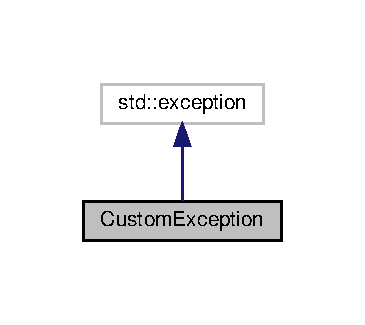
\includegraphics[width=175pt]{classCustomException__inherit__graph}
\end{center}
\end{figure}


Collaboration diagram for Custom\+Exception\+:\nopagebreak
\begin{figure}[H]
\begin{center}
\leavevmode
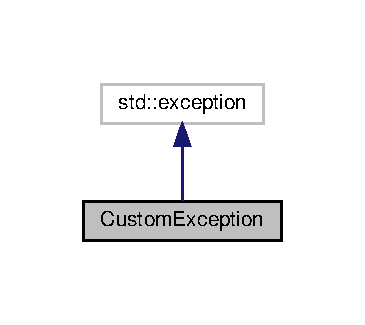
\includegraphics[width=175pt]{classCustomException__coll__graph}
\end{center}
\end{figure}
\subsection*{Public Member Functions}
\begin{DoxyCompactItemize}
\item 
\hyperlink{classCustomException_a07dbd163547759b7390b6f4588fff5a8}{Custom\+Exception} (const std\+::string \&msg=\char`\"{}Error\char`\"{})
\begin{DoxyCompactList}\small\item\em The default constructor which can set the internal message. \end{DoxyCompactList}\item 
void \hyperlink{classCustomException_a54289001348effb40f5780bb7f263abb}{Set\+Message} (const std\+::string \&msg)
\begin{DoxyCompactList}\small\item\em The aim of this function is to modify the internal message of the exception. \end{DoxyCompactList}\item 
void \hyperlink{classCustomException_ab8885c65813f31562bccdcce422b798c}{Append} (const std\+::string \&msg)
\begin{DoxyCompactList}\small\item\em This function is intended to add some text at the end of the internal message. \end{DoxyCompactList}\item 
\mbox{\Hypertarget{classCustomException_a0bb1756d6073f5bb8b6f1486b08fa5da}\label{classCustomException_a0bb1756d6073f5bb8b6f1486b08fa5da}} 
const char $\ast$ \hyperlink{classCustomException_a0bb1756d6073f5bb8b6f1486b08fa5da}{what} () const  throw ()
\begin{DoxyCompactList}\small\item\em This is a generic function for classes which manage exceptions and is intended to return the internal message as a C string ({\ttfamily char$\ast$}). \end{DoxyCompactList}\end{DoxyCompactItemize}


\subsection{Detailed Description}
A class derived from standard class {\ttfamily std\+::exception}. 

This class is customized to managed the exceptions in a desired way. This class has been defined to ease the appending of data to the message carried by an exception object. 

\subsection{Constructor \& Destructor Documentation}
\mbox{\Hypertarget{classCustomException_a07dbd163547759b7390b6f4588fff5a8}\label{classCustomException_a07dbd163547759b7390b6f4588fff5a8}} 
\index{Custom\+Exception@{Custom\+Exception}!Custom\+Exception@{Custom\+Exception}}
\index{Custom\+Exception@{Custom\+Exception}!Custom\+Exception@{Custom\+Exception}}
\subsubsection{\texorpdfstring{Custom\+Exception()}{CustomException()}}
{\footnotesize\ttfamily Custom\+Exception\+::\+Custom\+Exception (\begin{DoxyParamCaption}\item[{const std\+::string \&}]{msg = {\ttfamily \char`\"{}Error\char`\"{}} }\end{DoxyParamCaption})\hspace{0.3cm}{\ttfamily [inline]}}



The default constructor which can set the internal message. 


\begin{DoxyParams}[1]{Parameters}
\mbox{\tt in}  & {\em msg} & The internal message of the exception, which can be of type {\ttfamily char$\ast$} or {\ttfamily std\+::string}. \\
\hline
\end{DoxyParams}


\subsection{Member Function Documentation}
\mbox{\Hypertarget{classCustomException_ab8885c65813f31562bccdcce422b798c}\label{classCustomException_ab8885c65813f31562bccdcce422b798c}} 
\index{Custom\+Exception@{Custom\+Exception}!Append@{Append}}
\index{Append@{Append}!Custom\+Exception@{Custom\+Exception}}
\subsubsection{\texorpdfstring{Append()}{Append()}}
{\footnotesize\ttfamily void Custom\+Exception\+::\+Append (\begin{DoxyParamCaption}\item[{const std\+::string \&}]{msg }\end{DoxyParamCaption})\hspace{0.3cm}{\ttfamily [inline]}}



This function is intended to add some text at the end of the internal message. 


\begin{DoxyParams}[1]{Parameters}
\mbox{\tt in}  & {\em msg} & A sentence which must be appended to the internal message of the exception and which can be of type {\ttfamily char$\ast$} or {\ttfamily std\+::string}. \\
\hline
\end{DoxyParams}
\mbox{\Hypertarget{classCustomException_a54289001348effb40f5780bb7f263abb}\label{classCustomException_a54289001348effb40f5780bb7f263abb}} 
\index{Custom\+Exception@{Custom\+Exception}!Set\+Message@{Set\+Message}}
\index{Set\+Message@{Set\+Message}!Custom\+Exception@{Custom\+Exception}}
\subsubsection{\texorpdfstring{Set\+Message()}{SetMessage()}}
{\footnotesize\ttfamily void Custom\+Exception\+::\+Set\+Message (\begin{DoxyParamCaption}\item[{const std\+::string \&}]{msg }\end{DoxyParamCaption})\hspace{0.3cm}{\ttfamily [inline]}}



The aim of this function is to modify the internal message of the exception. 


\begin{DoxyParams}[1]{Parameters}
\mbox{\tt in}  & {\em msg} & The internal message of the exception, which can be of type {\ttfamily char$\ast$} or {\ttfamily std\+::string}. \\
\hline
\end{DoxyParams}


The documentation for this class was generated from the following file\+:\begin{DoxyCompactItemize}
\item 
\hyperlink{Basics_8h}{Basics.\+h}\end{DoxyCompactItemize}

\hypertarget{structFreqValues}{}\section{Freq\+Values Struct Reference}
\label{structFreqValues}\index{Freq\+Values@{Freq\+Values}}


The aim of this structure is to store the curve of a determined parameter or variable versus the frequency, which is named a frequency curve here.  




{\ttfamily \#include $<$Basics.\+h$>$}



Inheritance diagram for Freq\+Values\+:\nopagebreak
\begin{figure}[H]
\begin{center}
\leavevmode
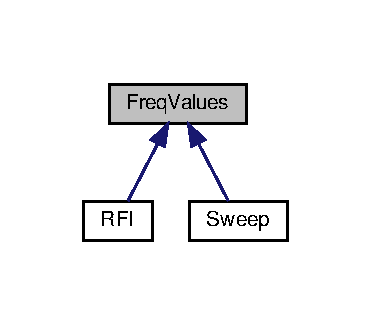
\includegraphics[width=178pt]{structFreqValues__inherit__graph}
\end{center}
\end{figure}


Collaboration diagram for Freq\+Values\+:\nopagebreak
\begin{figure}[H]
\begin{center}
\leavevmode
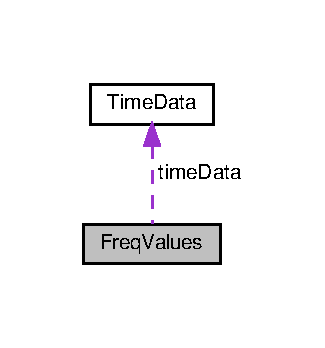
\includegraphics[width=156pt]{structFreqValues__coll__graph}
\end{center}
\end{figure}
\subsection*{Public Member Functions}
\begin{DoxyCompactItemize}
\item 
\hyperlink{structFreqValues_ab2ff89efb4571a8f6748017c6191d81e}{Freq\+Values} (const std\+::string \&typ=\char`\"{}unknown\char`\"{})
\begin{DoxyCompactList}\small\item\em The default constructor which can receive the curve type. \end{DoxyCompactList}\item 
\hyperlink{structFreqValues_a7061709cf9faa8e7ee6cf2d15fd30a66}{Freq\+Values} (const \hyperlink{structFreqValues}{Freq\+Values} \&freq\+Values)
\begin{DoxyCompactList}\small\item\em The copy constructor. \end{DoxyCompactList}\item 
\mbox{\Hypertarget{structFreqValues_a6ec6ba96834034b3b91d1519b90027b7}\label{structFreqValues_a6ec6ba96834034b3b91d1519b90027b7}} 
virtual \hyperlink{structFreqValues_a6ec6ba96834034b3b91d1519b90027b7}{$\sim$\+Freq\+Values} ()
\begin{DoxyCompactList}\small\item\em This is the structure\textquotesingle{}s destructor which is virtual because there are structures derived from this structure. \end{DoxyCompactList}\item 
bool \hyperlink{structFreqValues_a01315cf6bb4ed4e21ee1b6441c44a850}{Push\+Back} (const \hyperlink{structFreqValues}{Freq\+Values} \&freq\+Values)
\begin{DoxyCompactList}\small\item\em This method is intended to insert one data point (frequency,value) or a set of data points in the structure, at the end. \end{DoxyCompactList}\item 
\mbox{\Hypertarget{structFreqValues_ad47dd37005ced2182e9be2a1e16cd702}\label{structFreqValues_ad47dd37005ced2182e9be2a1e16cd702}} 
virtual void \hyperlink{structFreqValues_ad47dd37005ced2182e9be2a1e16cd702}{Clear} ()
\begin{DoxyCompactList}\small\item\em This method is intended to clear the structure, i.\+e. to delete all its data points. \end{DoxyCompactList}\item 
\mbox{\Hypertarget{structFreqValues_ae5a9b788cbf75ad4c3e1dd1ed86a0ddc}\label{structFreqValues_ae5a9b788cbf75ad4c3e1dd1ed86a0ddc}} 
bool \hyperlink{structFreqValues_ae5a9b788cbf75ad4c3e1dd1ed86a0ddc}{Empty} () const
\begin{DoxyCompactList}\small\item\em This method allows to know if the structure is empty, i.\+e. it has no data points. \end{DoxyCompactList}\item 
const \hyperlink{structFreqValues}{Freq\+Values} \& \hyperlink{structFreqValues_a11021e293ec300860ffc503d3c37a58c}{operator=} (const \hyperlink{structFreqValues}{Freq\+Values} \&freq\+Values)
\begin{DoxyCompactList}\small\item\em An overloading of the assignment operator adapted for this structure. \end{DoxyCompactList}\item 
const \hyperlink{structFreqValues}{Freq\+Values} \& \hyperlink{structFreqValues_a8024942907aaf5fd4aaa49850bbe6cd5}{operator+=} (const \hyperlink{structFreqValues}{Freq\+Values} \&rhs)
\begin{DoxyCompactList}\small\item\em An overloading of the operator += adapted for this structure. \end{DoxyCompactList}\item 
\mbox{\Hypertarget{structFreqValues_a954b961f99175f11f09d1cd5d834c545}\label{structFreqValues_a954b961f99175f11f09d1cd5d834c545}} 
float \hyperlink{structFreqValues_a954b961f99175f11f09d1cd5d834c545}{Mean\+Value} () const
\begin{DoxyCompactList}\small\item\em The aim of this method is to offer the mean value of all data points, i.\+e. it calculates the average. \end{DoxyCompactList}\end{DoxyCompactItemize}
\subsection*{Public Attributes}
\begin{DoxyCompactItemize}
\item 
\mbox{\Hypertarget{structFreqValues_a457f391fad53ee1e8bca839dde90c5f1}\label{structFreqValues_a457f391fad53ee1e8bca839dde90c5f1}} 
std\+::string \hyperlink{structFreqValues_a457f391fad53ee1e8bca839dde90c5f1}{type}
\begin{DoxyCompactList}\small\item\em Type of frequency values\+: ”sweep”, “frequency response”, “calibration curve”, “threshold curve”, “rfi", etc. \end{DoxyCompactList}\item 
\mbox{\Hypertarget{structFreqValues_a07669bbe3b65cbfb80300631ce85fb76}\label{structFreqValues_a07669bbe3b65cbfb80300631ce85fb76}} 
std\+::vector$<$ float $>$ \hyperlink{structFreqValues_a07669bbe3b65cbfb80300631ce85fb76}{values}
\begin{DoxyCompactList}\small\item\em RF power values (d\+Bm), gain values (dB or d\+Bi), noise figure values (dB), etc. \end{DoxyCompactList}\item 
\mbox{\Hypertarget{structFreqValues_a2b625831a46019f93a0999c1bed5c3a0}\label{structFreqValues_a2b625831a46019f93a0999c1bed5c3a0}} 
std\+::vector$<$ std\+::uint\+\_\+least64\+\_\+t $>$ \hyperlink{structFreqValues_a2b625831a46019f93a0999c1bed5c3a0}{frequencies}
\begin{DoxyCompactList}\small\item\em Frequency values in Hz. \end{DoxyCompactList}\item 
\hyperlink{structTimeData}{Time\+Data} \hyperlink{structFreqValues_a4c97a4710c83078f5af5d92f2bedfe61}{time\+Data}
\end{DoxyCompactItemize}
\subsection*{Friends}
\begin{DoxyCompactItemize}
\item 
\hyperlink{structFreqValues}{Freq\+Values} \hyperlink{structFreqValues_af2d38eb1ad1d3c6dfab8b4ea399c867d}{operator-\/} (const \hyperlink{structFreqValues}{Freq\+Values} \&argument)
\begin{DoxyCompactList}\small\item\em An overloading of the unary operator -\/ which negates a {\itshape \hyperlink{structFreqValues}{Freq\+Values}} object. \end{DoxyCompactList}\item 
\hyperlink{structFreqValues}{Freq\+Values} \hyperlink{structFreqValues_aa27b2370e9b314e6e0f308f4efb39a2f}{operator+} (const \hyperlink{structFreqValues}{Freq\+Values} \&lhs, const \hyperlink{structFreqValues}{Freq\+Values} \&rhs)
\begin{DoxyCompactList}\small\item\em An overloading of operator + which calculates the sum of two objects of structure {\itshape \hyperlink{structFreqValues}{Freq\+Values}}. \end{DoxyCompactList}\item 
\hyperlink{structFreqValues}{Freq\+Values} \hyperlink{structFreqValues_afa29d8e6cf56d1c724c712bcc95c0e4b}{operator+} (const \hyperlink{structFreqValues}{Freq\+Values} \&lhs, const float rhs)
\begin{DoxyCompactList}\small\item\em An overloading of operator + which calculates the sum of a {\itshape \hyperlink{structFreqValues}{Freq\+Values}} object and a {\itshape float} value, in that order. \end{DoxyCompactList}\item 
\hyperlink{structFreqValues}{Freq\+Values} \hyperlink{structFreqValues_add1a78bbae864d4a24ac7b491ae41b2e}{operator+} (const float lhs, const \hyperlink{structFreqValues}{Freq\+Values} \&rhs)
\begin{DoxyCompactList}\small\item\em An overloading of operator + which calculates the sum of a {\itshape float} value and a {\itshape \hyperlink{structFreqValues}{Freq\+Values}} object, in that order. \end{DoxyCompactList}\item 
\hyperlink{structFreqValues}{Freq\+Values} \hyperlink{structFreqValues_a05184c79e4dadc7a4e1f3a76fba1c3c8}{operator-\/} (const \hyperlink{structFreqValues}{Freq\+Values} \&lhs, const \hyperlink{structFreqValues}{Freq\+Values} \&rhs)
\begin{DoxyCompactList}\small\item\em An overloading of operator -\/ which calculates the subtraction of two objects of structure {\itshape \hyperlink{structFreqValues}{Freq\+Values}}. \end{DoxyCompactList}\item 
\hyperlink{structFreqValues}{Freq\+Values} \hyperlink{structFreqValues_ade558a5146a3dbea46f85e64d959ff3d}{operator-\/} (const \hyperlink{structFreqValues}{Freq\+Values} \&lhs, const float rhs)
\begin{DoxyCompactList}\small\item\em An overloading of operator -\/ which calculates the subtraction of a {\itshape \hyperlink{structFreqValues}{Freq\+Values}} object and a {\itshape float} value, in that order. \end{DoxyCompactList}\item 
\hyperlink{structFreqValues}{Freq\+Values} \hyperlink{structFreqValues_aa248d5bc83ba0c614137b042947064a8}{operator-\/} (const float lhs, const \hyperlink{structFreqValues}{Freq\+Values} \&rhs)
\begin{DoxyCompactList}\small\item\em An overloading of operator -\/ which calculates the subtraction of a {\itshape float} value and a {\itshape \hyperlink{structFreqValues}{Freq\+Values}} object, in that order. \end{DoxyCompactList}\item 
\hyperlink{structFreqValues}{Freq\+Values} \hyperlink{structFreqValues_a3e567844a5d4347e3b30e696132bfb7c}{operator$\ast$} (const \hyperlink{structFreqValues}{Freq\+Values} \&lhs, const \hyperlink{structFreqValues}{Freq\+Values} \&rhs)
\begin{DoxyCompactList}\small\item\em An overloading of operator $\ast$ which multiplies two objects of structure {\itshape \hyperlink{structFreqValues}{Freq\+Values}}. \end{DoxyCompactList}\item 
\hyperlink{structFreqValues}{Freq\+Values} \hyperlink{structFreqValues_aea565aadf51307e09845c72179e5082d}{operator$\ast$} (const \hyperlink{structFreqValues}{Freq\+Values} \&lhs, const float rhs)
\begin{DoxyCompactList}\small\item\em An overloading of operator $\ast$ which multiplies a {\itshape \hyperlink{structFreqValues}{Freq\+Values}} object and a {\itshape float} value, in that order. \end{DoxyCompactList}\item 
\hyperlink{structFreqValues}{Freq\+Values} \hyperlink{structFreqValues_ab9bb62425b97f45a5eb485cf745bfe4a}{operator$\ast$} (const float lhs, const \hyperlink{structFreqValues}{Freq\+Values} \&rhs)
\begin{DoxyCompactList}\small\item\em An overloading of operator $\ast$ which multiplies a {\itshape float} value and a {\itshape \hyperlink{structFreqValues}{Freq\+Values}} object, in that order. \end{DoxyCompactList}\item 
\hyperlink{structFreqValues}{Freq\+Values} \hyperlink{structFreqValues_a26f13922dd72ad292bea45072abc2c96}{operator/} (const \hyperlink{structFreqValues}{Freq\+Values} \&lhs, const \hyperlink{structFreqValues}{Freq\+Values} \&rhs)
\begin{DoxyCompactList}\small\item\em An overloading of operator / which calculates the division between two objects of structure {\itshape \hyperlink{structFreqValues}{Freq\+Values}}. \end{DoxyCompactList}\item 
\hyperlink{structFreqValues}{Freq\+Values} \hyperlink{structFreqValues_a392b5ed122a4deafa3ba773f4829c20a}{operator/} (const \hyperlink{structFreqValues}{Freq\+Values} \&lhs, const float rhs)
\begin{DoxyCompactList}\small\item\em An overloading of operator / which calculates the division between a {\itshape \hyperlink{structFreqValues}{Freq\+Values}} object and a {\itshape float} value, in that order. \end{DoxyCompactList}\item 
\hyperlink{structFreqValues}{Freq\+Values} \hyperlink{structFreqValues_aed1d809f52aa8f6da3afa2af8a45d288}{operator/} (const float lhs, const \hyperlink{structFreqValues}{Freq\+Values} \&rhs)
\begin{DoxyCompactList}\small\item\em An overloading of operator / which calculates the division between a {\itshape float} value and a {\itshape \hyperlink{structFreqValues}{Freq\+Values}} object, in that order. \end{DoxyCompactList}\item 
\hyperlink{structFreqValues}{Freq\+Values} \hyperlink{structFreqValues_a90781867604621a99e59d4fcdc4a5f38}{log10} (const \hyperlink{structFreqValues}{Freq\+Values} \&argument)
\begin{DoxyCompactList}\small\item\em An overloading of function {\ttfamily \hyperlink{structFreqValues_a90781867604621a99e59d4fcdc4a5f38}{log10()}}, decimal logarithm, adapted to receive an argument of type {\itshape \hyperlink{structFreqValues}{Freq\+Values}}. \end{DoxyCompactList}\item 
\hyperlink{structFreqValues}{Freq\+Values} \hyperlink{structFreqValues_a8b8ee90b9d108ad7008a3613b31253e7}{pow} (const \hyperlink{structFreqValues}{Freq\+Values} \&base, const float exponent)
\begin{DoxyCompactList}\small\item\em An overloading of function {\ttfamily \hyperlink{structFreqValues_a8b8ee90b9d108ad7008a3613b31253e7}{pow()}}, power function, adapted to receive an argument of type {\itshape \hyperlink{structFreqValues}{Freq\+Values}} as base and an argument of type {\itshape float} as exponent. \end{DoxyCompactList}\item 
\hyperlink{structFreqValues}{Freq\+Values} \hyperlink{structFreqValues_a4a50ddd9aa3d48c0b3da456ca07551a5}{pow} (const float base, const \hyperlink{structFreqValues}{Freq\+Values} \&exponent)
\begin{DoxyCompactList}\small\item\em An overloading of function {\ttfamily \hyperlink{structFreqValues_a8b8ee90b9d108ad7008a3613b31253e7}{pow()}}, exponentiation, adapted to receive an argument of type {\itshape float} as base and an argument of type {\itshape \hyperlink{structFreqValues}{Freq\+Values}} as exponent. \end{DoxyCompactList}\end{DoxyCompactItemize}


\subsection{Detailed Description}
The aim of this structure is to store the curve of a determined parameter or variable versus the frequency, which is named a frequency curve here. 

\subsection{Constructor \& Destructor Documentation}
\mbox{\Hypertarget{structFreqValues_ab2ff89efb4571a8f6748017c6191d81e}\label{structFreqValues_ab2ff89efb4571a8f6748017c6191d81e}} 
\index{Freq\+Values@{Freq\+Values}!Freq\+Values@{Freq\+Values}}
\index{Freq\+Values@{Freq\+Values}!Freq\+Values@{Freq\+Values}}
\subsubsection{\texorpdfstring{Freq\+Values()}{FreqValues()}\hspace{0.1cm}{\footnotesize\ttfamily [1/2]}}
{\footnotesize\ttfamily Freq\+Values\+::\+Freq\+Values (\begin{DoxyParamCaption}\item[{const std\+::string \&}]{typ = {\ttfamily \char`\"{}unknown\char`\"{}} }\end{DoxyParamCaption})\hspace{0.3cm}{\ttfamily [inline]}}



The default constructor which can receive the curve type. 


\begin{DoxyParams}[1]{Parameters}
\mbox{\tt in}  & {\em typ} & The type of parameter whose curve of values versus frequency is stored in the structure. \\
\hline
\end{DoxyParams}
\mbox{\Hypertarget{structFreqValues_a7061709cf9faa8e7ee6cf2d15fd30a66}\label{structFreqValues_a7061709cf9faa8e7ee6cf2d15fd30a66}} 
\index{Freq\+Values@{Freq\+Values}!Freq\+Values@{Freq\+Values}}
\index{Freq\+Values@{Freq\+Values}!Freq\+Values@{Freq\+Values}}
\subsubsection{\texorpdfstring{Freq\+Values()}{FreqValues()}\hspace{0.1cm}{\footnotesize\ttfamily [2/2]}}
{\footnotesize\ttfamily Freq\+Values\+::\+Freq\+Values (\begin{DoxyParamCaption}\item[{const \hyperlink{structFreqValues}{Freq\+Values} \&}]{freq\+Values }\end{DoxyParamCaption})\hspace{0.3cm}{\ttfamily [inline]}}



The copy constructor. 


\begin{DoxyParams}[1]{Parameters}
\mbox{\tt in}  & {\em freq\+Values} & Another {\itshape \hyperlink{structFreqValues}{Freq\+Values}} structure which is given to copy its attributes. \\
\hline
\end{DoxyParams}


\subsection{Member Function Documentation}
\mbox{\Hypertarget{structFreqValues_a8024942907aaf5fd4aaa49850bbe6cd5}\label{structFreqValues_a8024942907aaf5fd4aaa49850bbe6cd5}} 
\index{Freq\+Values@{Freq\+Values}!operator+=@{operator+=}}
\index{operator+=@{operator+=}!Freq\+Values@{Freq\+Values}}
\subsubsection{\texorpdfstring{operator+=()}{operator+=()}}
{\footnotesize\ttfamily const \hyperlink{structFreqValues}{Freq\+Values} \& Freq\+Values\+::operator+= (\begin{DoxyParamCaption}\item[{const \hyperlink{structFreqValues}{Freq\+Values} \&}]{rhs }\end{DoxyParamCaption})}



An overloading of the operator += adapted for this structure. 

This method is not intended to concatenate two {\itshape \hyperlink{structFreqValues}{Freq\+Values}} structure, what is performed by the method {\ttfamily \hyperlink{structFreqValues_a01315cf6bb4ed4e21ee1b6441c44a850}{Push\+Back()}}, but its aim is to sum each point of base structure with the corresponding point of the structure given as argument, and to save the results in the base structure.

The method returns a {\ttfamily const} reference to the base structure. 
\begin{DoxyParams}[1]{Parameters}
\mbox{\tt in}  & {\em rhs} & A {\itshape \hyperlink{structFreqValues}{Freq\+Values}} structure which is given to perform the sum. \\
\hline
\end{DoxyParams}
\mbox{\Hypertarget{structFreqValues_a11021e293ec300860ffc503d3c37a58c}\label{structFreqValues_a11021e293ec300860ffc503d3c37a58c}} 
\index{Freq\+Values@{Freq\+Values}!operator=@{operator=}}
\index{operator=@{operator=}!Freq\+Values@{Freq\+Values}}
\subsubsection{\texorpdfstring{operator=()}{operator=()}}
{\footnotesize\ttfamily const \hyperlink{structFreqValues}{Freq\+Values} \& Freq\+Values\+::operator= (\begin{DoxyParamCaption}\item[{const \hyperlink{structFreqValues}{Freq\+Values} \&}]{freq\+Values }\end{DoxyParamCaption})}



An overloading of the assignment operator adapted for this structure. 

The method returns a {\ttfamily const} reference to the base structure. 
\begin{DoxyParams}[1]{Parameters}
\mbox{\tt in}  & {\em freq\+Values} & Another {\itshape \hyperlink{structFreqValues}{Freq\+Values}} structure which is given to copy its attributes. \\
\hline
\end{DoxyParams}
\mbox{\Hypertarget{structFreqValues_a01315cf6bb4ed4e21ee1b6441c44a850}\label{structFreqValues_a01315cf6bb4ed4e21ee1b6441c44a850}} 
\index{Freq\+Values@{Freq\+Values}!Push\+Back@{Push\+Back}}
\index{Push\+Back@{Push\+Back}!Freq\+Values@{Freq\+Values}}
\subsubsection{\texorpdfstring{Push\+Back()}{PushBack()}}
{\footnotesize\ttfamily bool Freq\+Values\+::\+Push\+Back (\begin{DoxyParamCaption}\item[{const \hyperlink{structFreqValues}{Freq\+Values} \&}]{freq\+Values }\end{DoxyParamCaption})}



This method is intended to insert one data point (frequency,value) or a set of data points in the structure, at the end. 


\begin{DoxyParams}[1]{Parameters}
\mbox{\tt in}  & {\em freq\+Values} & Another {\itshape \hyperlink{structFreqValues}{Freq\+Values}} structure whose values must be inserted at the end of this structure. \\
\hline
\end{DoxyParams}


\subsection{Friends And Related Function Documentation}
\mbox{\Hypertarget{structFreqValues_a90781867604621a99e59d4fcdc4a5f38}\label{structFreqValues_a90781867604621a99e59d4fcdc4a5f38}} 
\index{Freq\+Values@{Freq\+Values}!log10@{log10}}
\index{log10@{log10}!Freq\+Values@{Freq\+Values}}
\subsubsection{\texorpdfstring{log10}{log10}}
{\footnotesize\ttfamily \hyperlink{structFreqValues}{Freq\+Values} log10 (\begin{DoxyParamCaption}\item[{const \hyperlink{structFreqValues}{Freq\+Values} \&}]{argument }\end{DoxyParamCaption})\hspace{0.3cm}{\ttfamily [friend]}}



An overloading of function {\ttfamily \hyperlink{structFreqValues_a90781867604621a99e59d4fcdc4a5f38}{log10()}}, decimal logarithm, adapted to receive an argument of type {\itshape \hyperlink{structFreqValues}{Freq\+Values}}. 

This function takes each point of the given structure, apply the decimal logarithm whit its value and stores the result in a different {\itshape \hyperlink{structFreqValues}{Freq\+Values}} structure, which is then returned. The rest of attributes (frequency, type, timestamp, etc.) are copied as-\/is to the object to be returned. 
\begin{DoxyParams}[1]{Parameters}
\mbox{\tt in}  & {\em argument} & The {\itshape \hyperlink{structFreqValues}{Freq\+Values}} structure to be used as argument to the decimal logarithm operation. \\
\hline
\end{DoxyParams}
\mbox{\Hypertarget{structFreqValues_a3e567844a5d4347e3b30e696132bfb7c}\label{structFreqValues_a3e567844a5d4347e3b30e696132bfb7c}} 
\index{Freq\+Values@{Freq\+Values}!operator$\ast$@{operator$\ast$}}
\index{operator$\ast$@{operator$\ast$}!Freq\+Values@{Freq\+Values}}
\subsubsection{\texorpdfstring{operator$\ast$}{operator*}\hspace{0.1cm}{\footnotesize\ttfamily [1/3]}}
{\footnotesize\ttfamily \hyperlink{structFreqValues}{Freq\+Values} operator$\ast$ (\begin{DoxyParamCaption}\item[{const \hyperlink{structFreqValues}{Freq\+Values} \&}]{lhs,  }\item[{const \hyperlink{structFreqValues}{Freq\+Values} \&}]{rhs }\end{DoxyParamCaption})\hspace{0.3cm}{\ttfamily [friend]}}



An overloading of operator $\ast$ which multiplies two objects of structure {\itshape \hyperlink{structFreqValues}{Freq\+Values}}. 

Before performing the operation, the function checks if the frequencies of each structure match and if the \char`\"{}values\char`\"{} vectors have the same sizes as the \char`\"{}frequencies\char`\"{} vectors. The values of the of object to be returned are determined by the operation, while the rest of attributes (frequency, type, timestamp, etc.) are copied from the left-\/hand side argument.

The function returns a {\itshape \hyperlink{structFreqValues}{Freq\+Values}} object with the results of the operation. 
\begin{DoxyParams}[1]{Parameters}
\mbox{\tt in}  & {\em lhs} & The left-\/hand side operand. \\
\hline
\mbox{\tt in}  & {\em rhs} & The right-\/hand side operand. \\
\hline
\end{DoxyParams}
\mbox{\Hypertarget{structFreqValues_aea565aadf51307e09845c72179e5082d}\label{structFreqValues_aea565aadf51307e09845c72179e5082d}} 
\index{Freq\+Values@{Freq\+Values}!operator$\ast$@{operator$\ast$}}
\index{operator$\ast$@{operator$\ast$}!Freq\+Values@{Freq\+Values}}
\subsubsection{\texorpdfstring{operator$\ast$}{operator*}\hspace{0.1cm}{\footnotesize\ttfamily [2/3]}}
{\footnotesize\ttfamily \hyperlink{structFreqValues}{Freq\+Values} operator$\ast$ (\begin{DoxyParamCaption}\item[{const \hyperlink{structFreqValues}{Freq\+Values} \&}]{lhs,  }\item[{const float}]{rhs }\end{DoxyParamCaption})\hspace{0.3cm}{\ttfamily [friend]}}



An overloading of operator $\ast$ which multiplies a {\itshape \hyperlink{structFreqValues}{Freq\+Values}} object and a {\itshape float} value, in that order. 

This function calls the function {\ttfamily operator$\ast$(float,\+Freq\+Values)} with the order of its argument inverted, taking into account the commutative property of the multiplication.

The function returns a {\itshape \hyperlink{structFreqValues}{Freq\+Values}} object with the results of the operation. 
\begin{DoxyParams}[1]{Parameters}
\mbox{\tt in}  & {\em lhs} & The left-\/hand side operand. \\
\hline
\mbox{\tt in}  & {\em rhs} & The right-\/hand side operand. \\
\hline
\end{DoxyParams}
\mbox{\Hypertarget{structFreqValues_ab9bb62425b97f45a5eb485cf745bfe4a}\label{structFreqValues_ab9bb62425b97f45a5eb485cf745bfe4a}} 
\index{Freq\+Values@{Freq\+Values}!operator$\ast$@{operator$\ast$}}
\index{operator$\ast$@{operator$\ast$}!Freq\+Values@{Freq\+Values}}
\subsubsection{\texorpdfstring{operator$\ast$}{operator*}\hspace{0.1cm}{\footnotesize\ttfamily [3/3]}}
{\footnotesize\ttfamily \hyperlink{structFreqValues}{Freq\+Values} operator$\ast$ (\begin{DoxyParamCaption}\item[{const float}]{lhs,  }\item[{const \hyperlink{structFreqValues}{Freq\+Values} \&}]{rhs }\end{DoxyParamCaption})\hspace{0.3cm}{\ttfamily [friend]}}



An overloading of operator $\ast$ which multiplies a {\itshape float} value and a {\itshape \hyperlink{structFreqValues}{Freq\+Values}} object, in that order. 

The values of the object to be returned are determined by the operation, while the rest of attributes (frequency, type, timestamp, etc.) are copied from the right-\/hand argument, which is the only argument that is of type {\itshape \hyperlink{structFreqValues}{Freq\+Values}}.

The function returns a {\itshape \hyperlink{structFreqValues}{Freq\+Values}} object with the results of the operation. 
\begin{DoxyParams}[1]{Parameters}
\mbox{\tt in}  & {\em lhs} & The left-\/hand side operand. \\
\hline
\mbox{\tt in}  & {\em rhs} & The right-\/hand side operand. \\
\hline
\end{DoxyParams}
\mbox{\Hypertarget{structFreqValues_aa27b2370e9b314e6e0f308f4efb39a2f}\label{structFreqValues_aa27b2370e9b314e6e0f308f4efb39a2f}} 
\index{Freq\+Values@{Freq\+Values}!operator+@{operator+}}
\index{operator+@{operator+}!Freq\+Values@{Freq\+Values}}
\subsubsection{\texorpdfstring{operator+}{operator+}\hspace{0.1cm}{\footnotesize\ttfamily [1/3]}}
{\footnotesize\ttfamily \hyperlink{structFreqValues}{Freq\+Values} operator+ (\begin{DoxyParamCaption}\item[{const \hyperlink{structFreqValues}{Freq\+Values} \&}]{lhs,  }\item[{const \hyperlink{structFreqValues}{Freq\+Values} \&}]{rhs }\end{DoxyParamCaption})\hspace{0.3cm}{\ttfamily [friend]}}



An overloading of operator + which calculates the sum of two objects of structure {\itshape \hyperlink{structFreqValues}{Freq\+Values}}. 

Before performing the operation, the function checks if the frequencies of each structure match and if the \char`\"{}values\char`\"{} vectors have the same sizes as the \char`\"{}frequencies\char`\"{} vectors. The values of the of object to be returned are determined by the operation, while the rest of attributes (frequency, type, timestamp, etc.) are copied from the left-\/hand side argument.

The function returns a {\itshape \hyperlink{structFreqValues}{Freq\+Values}} object with the results of the operation. 
\begin{DoxyParams}[1]{Parameters}
\mbox{\tt in}  & {\em lhs} & The left-\/hand side operand. \\
\hline
\mbox{\tt in}  & {\em rhs} & The right-\/hand side operand. \\
\hline
\end{DoxyParams}
\mbox{\Hypertarget{structFreqValues_afa29d8e6cf56d1c724c712bcc95c0e4b}\label{structFreqValues_afa29d8e6cf56d1c724c712bcc95c0e4b}} 
\index{Freq\+Values@{Freq\+Values}!operator+@{operator+}}
\index{operator+@{operator+}!Freq\+Values@{Freq\+Values}}
\subsubsection{\texorpdfstring{operator+}{operator+}\hspace{0.1cm}{\footnotesize\ttfamily [2/3]}}
{\footnotesize\ttfamily \hyperlink{structFreqValues}{Freq\+Values} operator+ (\begin{DoxyParamCaption}\item[{const \hyperlink{structFreqValues}{Freq\+Values} \&}]{lhs,  }\item[{const float}]{rhs }\end{DoxyParamCaption})\hspace{0.3cm}{\ttfamily [friend]}}



An overloading of operator + which calculates the sum of a {\itshape \hyperlink{structFreqValues}{Freq\+Values}} object and a {\itshape float} value, in that order. 

The values of the of object to be returned are determined by the operation, while the rest of attributes (frequency, type, timestamp, etc.) are copied from the left-\/hand side argument, which is the only argument that is of type {\itshape \hyperlink{structFreqValues}{Freq\+Values}}.

The function returns a {\itshape \hyperlink{structFreqValues}{Freq\+Values}} object with the results of the operation. 
\begin{DoxyParams}[1]{Parameters}
\mbox{\tt in}  & {\em lhs} & The left-\/hand side operand. \\
\hline
\mbox{\tt in}  & {\em rhs} & The right-\/hand side operand. \\
\hline
\end{DoxyParams}
\mbox{\Hypertarget{structFreqValues_add1a78bbae864d4a24ac7b491ae41b2e}\label{structFreqValues_add1a78bbae864d4a24ac7b491ae41b2e}} 
\index{Freq\+Values@{Freq\+Values}!operator+@{operator+}}
\index{operator+@{operator+}!Freq\+Values@{Freq\+Values}}
\subsubsection{\texorpdfstring{operator+}{operator+}\hspace{0.1cm}{\footnotesize\ttfamily [3/3]}}
{\footnotesize\ttfamily \hyperlink{structFreqValues}{Freq\+Values} operator+ (\begin{DoxyParamCaption}\item[{const float}]{lhs,  }\item[{const \hyperlink{structFreqValues}{Freq\+Values} \&}]{rhs }\end{DoxyParamCaption})\hspace{0.3cm}{\ttfamily [friend]}}



An overloading of operator + which calculates the sum of a {\itshape float} value and a {\itshape \hyperlink{structFreqValues}{Freq\+Values}} object, in that order. 

This function calls the function {\ttfamily operator+(\+Freq\+Values,float)} with the order of its arguments inverted, taking into account the commutative property of the sum. The values of the of object to be returned are determined by the operation, while the rest of attributes (frequency, type, timestamp, etc.) are copied from the right-\/hand side argument, which is the only argument that is of type {\itshape \hyperlink{structFreqValues}{Freq\+Values}}.

The function returns a {\itshape \hyperlink{structFreqValues}{Freq\+Values}} object with the results of the operation. 
\begin{DoxyParams}[1]{Parameters}
\mbox{\tt in}  & {\em lhs} & The left-\/hand side operand. \\
\hline
\mbox{\tt in}  & {\em rhs} & The right-\/hand side operand. \\
\hline
\end{DoxyParams}
\mbox{\Hypertarget{structFreqValues_af2d38eb1ad1d3c6dfab8b4ea399c867d}\label{structFreqValues_af2d38eb1ad1d3c6dfab8b4ea399c867d}} 
\index{Freq\+Values@{Freq\+Values}!operator-\/@{operator-\/}}
\index{operator-\/@{operator-\/}!Freq\+Values@{Freq\+Values}}
\subsubsection{\texorpdfstring{operator-\/}{operator-}\hspace{0.1cm}{\footnotesize\ttfamily [1/4]}}
{\footnotesize\ttfamily \hyperlink{structFreqValues}{Freq\+Values} operator-\/ (\begin{DoxyParamCaption}\item[{const \hyperlink{structFreqValues}{Freq\+Values} \&}]{argument }\end{DoxyParamCaption})\hspace{0.3cm}{\ttfamily [friend]}}



An overloading of the unary operator -\/ which negates a {\itshape \hyperlink{structFreqValues}{Freq\+Values}} object. 

This function takes each point of the given structure, negates it (the stored value, not the frequency) and stores the result in a different {\itshape \hyperlink{structFreqValues}{Freq\+Values}} structure, which is then returned. The rest of attributes (frequency, type, timestamp, etc.) are copied as-\/is to the object to be returned. 
\begin{DoxyParams}[1]{Parameters}
\mbox{\tt in}  & {\em argument} & The {\itshape \hyperlink{structFreqValues}{Freq\+Values}} structure to be negated. \\
\hline
\end{DoxyParams}
\mbox{\Hypertarget{structFreqValues_a05184c79e4dadc7a4e1f3a76fba1c3c8}\label{structFreqValues_a05184c79e4dadc7a4e1f3a76fba1c3c8}} 
\index{Freq\+Values@{Freq\+Values}!operator-\/@{operator-\/}}
\index{operator-\/@{operator-\/}!Freq\+Values@{Freq\+Values}}
\subsubsection{\texorpdfstring{operator-\/}{operator-}\hspace{0.1cm}{\footnotesize\ttfamily [2/4]}}
{\footnotesize\ttfamily \hyperlink{structFreqValues}{Freq\+Values} operator-\/ (\begin{DoxyParamCaption}\item[{const \hyperlink{structFreqValues}{Freq\+Values} \&}]{lhs,  }\item[{const \hyperlink{structFreqValues}{Freq\+Values} \&}]{rhs }\end{DoxyParamCaption})\hspace{0.3cm}{\ttfamily [friend]}}



An overloading of operator -\/ which calculates the subtraction of two objects of structure {\itshape \hyperlink{structFreqValues}{Freq\+Values}}. 

This function calls the function {\ttfamily operator+(\+Freq\+Values,\+Freq\+Values)} with the right-\/hand side operand negated.

The function returns a {\itshape \hyperlink{structFreqValues}{Freq\+Values}} object with the results of the operation. 
\begin{DoxyParams}[1]{Parameters}
\mbox{\tt in}  & {\em lhs} & The left-\/hand side operand. \\
\hline
\mbox{\tt in}  & {\em rhs} & The right-\/hand side operand. \\
\hline
\end{DoxyParams}
\mbox{\Hypertarget{structFreqValues_ade558a5146a3dbea46f85e64d959ff3d}\label{structFreqValues_ade558a5146a3dbea46f85e64d959ff3d}} 
\index{Freq\+Values@{Freq\+Values}!operator-\/@{operator-\/}}
\index{operator-\/@{operator-\/}!Freq\+Values@{Freq\+Values}}
\subsubsection{\texorpdfstring{operator-\/}{operator-}\hspace{0.1cm}{\footnotesize\ttfamily [3/4]}}
{\footnotesize\ttfamily \hyperlink{structFreqValues}{Freq\+Values} operator-\/ (\begin{DoxyParamCaption}\item[{const \hyperlink{structFreqValues}{Freq\+Values} \&}]{lhs,  }\item[{const float}]{rhs }\end{DoxyParamCaption})\hspace{0.3cm}{\ttfamily [friend]}}



An overloading of operator -\/ which calculates the subtraction of a {\itshape \hyperlink{structFreqValues}{Freq\+Values}} object and a {\itshape float} value, in that order. 

This function calls the function {\ttfamily operator+(\+Freq\+Values,float)} with the right-\/hand side operand negated.

The function returns a {\itshape \hyperlink{structFreqValues}{Freq\+Values}} object with the results of the operation. 
\begin{DoxyParams}[1]{Parameters}
\mbox{\tt in}  & {\em lhs} & The left-\/hand side operand. \\
\hline
\mbox{\tt in}  & {\em rhs} & The right-\/hand side operand. \\
\hline
\end{DoxyParams}
\mbox{\Hypertarget{structFreqValues_aa248d5bc83ba0c614137b042947064a8}\label{structFreqValues_aa248d5bc83ba0c614137b042947064a8}} 
\index{Freq\+Values@{Freq\+Values}!operator-\/@{operator-\/}}
\index{operator-\/@{operator-\/}!Freq\+Values@{Freq\+Values}}
\subsubsection{\texorpdfstring{operator-\/}{operator-}\hspace{0.1cm}{\footnotesize\ttfamily [4/4]}}
{\footnotesize\ttfamily \hyperlink{structFreqValues}{Freq\+Values} operator-\/ (\begin{DoxyParamCaption}\item[{const float}]{lhs,  }\item[{const \hyperlink{structFreqValues}{Freq\+Values} \&}]{rhs }\end{DoxyParamCaption})\hspace{0.3cm}{\ttfamily [friend]}}



An overloading of operator -\/ which calculates the subtraction of a {\itshape float} value and a {\itshape \hyperlink{structFreqValues}{Freq\+Values}} object, in that order. 

This function calls the function {\ttfamily operator+(float,\+Freq\+Values)} with the right-\/hand side operand negated.

The function returns a {\itshape \hyperlink{structFreqValues}{Freq\+Values}} object with the results of the operation. 
\begin{DoxyParams}[1]{Parameters}
\mbox{\tt in}  & {\em lhs} & The left-\/hand side operand. \\
\hline
\mbox{\tt in}  & {\em rhs} & The right-\/hand side operand. \\
\hline
\end{DoxyParams}
\mbox{\Hypertarget{structFreqValues_a26f13922dd72ad292bea45072abc2c96}\label{structFreqValues_a26f13922dd72ad292bea45072abc2c96}} 
\index{Freq\+Values@{Freq\+Values}!operator/@{operator/}}
\index{operator/@{operator/}!Freq\+Values@{Freq\+Values}}
\subsubsection{\texorpdfstring{operator/}{operator/}\hspace{0.1cm}{\footnotesize\ttfamily [1/3]}}
{\footnotesize\ttfamily \hyperlink{structFreqValues}{Freq\+Values} operator/ (\begin{DoxyParamCaption}\item[{const \hyperlink{structFreqValues}{Freq\+Values} \&}]{lhs,  }\item[{const \hyperlink{structFreqValues}{Freq\+Values} \&}]{rhs }\end{DoxyParamCaption})\hspace{0.3cm}{\ttfamily [friend]}}



An overloading of operator / which calculates the division between two objects of structure {\itshape \hyperlink{structFreqValues}{Freq\+Values}}. 

Before performing the operation, the function checks if the frequencies of each structure match and if the \char`\"{}values\char`\"{} vectors have the same sizes as the \char`\"{}frequencies\char`\"{} vectors. The values of the of object to be returned are determined by the operation, while the rest of attributes (frequency, type, timestamp, etc.) are copied from the left-\/hand side argument.

The function returns a {\itshape \hyperlink{structFreqValues}{Freq\+Values}} object with the results of the operation. 
\begin{DoxyParams}[1]{Parameters}
\mbox{\tt in}  & {\em lhs} & The left-\/hand side operand. \\
\hline
\mbox{\tt in}  & {\em rhs} & The right-\/hand side operand. \\
\hline
\end{DoxyParams}
\mbox{\Hypertarget{structFreqValues_a392b5ed122a4deafa3ba773f4829c20a}\label{structFreqValues_a392b5ed122a4deafa3ba773f4829c20a}} 
\index{Freq\+Values@{Freq\+Values}!operator/@{operator/}}
\index{operator/@{operator/}!Freq\+Values@{Freq\+Values}}
\subsubsection{\texorpdfstring{operator/}{operator/}\hspace{0.1cm}{\footnotesize\ttfamily [2/3]}}
{\footnotesize\ttfamily \hyperlink{structFreqValues}{Freq\+Values} operator/ (\begin{DoxyParamCaption}\item[{const \hyperlink{structFreqValues}{Freq\+Values} \&}]{lhs,  }\item[{const float}]{rhs }\end{DoxyParamCaption})\hspace{0.3cm}{\ttfamily [friend]}}



An overloading of operator / which calculates the division between a {\itshape \hyperlink{structFreqValues}{Freq\+Values}} object and a {\itshape float} value, in that order. 

This function calls the function {\ttfamily operator$\ast$(\+Freq\+Values,float)} wit the right-\/hand argument inverted.

The function returns a {\itshape \hyperlink{structFreqValues}{Freq\+Values}} object with the results of the operation. 
\begin{DoxyParams}[1]{Parameters}
\mbox{\tt in}  & {\em lhs} & The left-\/hand side operand. \\
\hline
\mbox{\tt in}  & {\em rhs} & The right-\/hand side operand. \\
\hline
\end{DoxyParams}
\mbox{\Hypertarget{structFreqValues_aed1d809f52aa8f6da3afa2af8a45d288}\label{structFreqValues_aed1d809f52aa8f6da3afa2af8a45d288}} 
\index{Freq\+Values@{Freq\+Values}!operator/@{operator/}}
\index{operator/@{operator/}!Freq\+Values@{Freq\+Values}}
\subsubsection{\texorpdfstring{operator/}{operator/}\hspace{0.1cm}{\footnotesize\ttfamily [3/3]}}
{\footnotesize\ttfamily \hyperlink{structFreqValues}{Freq\+Values} operator/ (\begin{DoxyParamCaption}\item[{const float}]{lhs,  }\item[{const \hyperlink{structFreqValues}{Freq\+Values} \&}]{rhs }\end{DoxyParamCaption})\hspace{0.3cm}{\ttfamily [friend]}}



An overloading of operator / which calculates the division between a {\itshape float} value and a {\itshape \hyperlink{structFreqValues}{Freq\+Values}} object, in that order. 

The values of the object to be returned are determined by the operation, while the rest of attributes (frequency, type, timestamp, etc.) are copied from the right-\/hand argument, which is the only argument that is of type {\itshape \hyperlink{structFreqValues}{Freq\+Values}}.

The function returns a {\itshape \hyperlink{structFreqValues}{Freq\+Values}} object with the results of the operation. 
\begin{DoxyParams}[1]{Parameters}
\mbox{\tt in}  & {\em lhs} & The left-\/hand side operand. \\
\hline
\mbox{\tt in}  & {\em rhs} & The right-\/hand side operand. \\
\hline
\end{DoxyParams}
\mbox{\Hypertarget{structFreqValues_a8b8ee90b9d108ad7008a3613b31253e7}\label{structFreqValues_a8b8ee90b9d108ad7008a3613b31253e7}} 
\index{Freq\+Values@{Freq\+Values}!pow@{pow}}
\index{pow@{pow}!Freq\+Values@{Freq\+Values}}
\subsubsection{\texorpdfstring{pow}{pow}\hspace{0.1cm}{\footnotesize\ttfamily [1/2]}}
{\footnotesize\ttfamily \hyperlink{structFreqValues}{Freq\+Values} pow (\begin{DoxyParamCaption}\item[{const \hyperlink{structFreqValues}{Freq\+Values} \&}]{base,  }\item[{const float}]{exponent }\end{DoxyParamCaption})\hspace{0.3cm}{\ttfamily [friend]}}



An overloading of function {\ttfamily \hyperlink{structFreqValues_a8b8ee90b9d108ad7008a3613b31253e7}{pow()}}, power function, adapted to receive an argument of type {\itshape \hyperlink{structFreqValues}{Freq\+Values}} as base and an argument of type {\itshape float} as exponent. 

This function takes each point of the structure, raises its value to the exponent and stores the result in a different {\itshape \hyperlink{structFreqValues}{Freq\+Values}} structure, which is then returned. The rest of attributes (frequency, type, timestamp, etc.) are copied from the left-\/hand side argument, which the only argument that is of type {\itshape \hyperlink{structFreqValues}{Freq\+Values}}. 
\begin{DoxyParams}[1]{Parameters}
\mbox{\tt in}  & {\em base} & The {\itshape \hyperlink{structFreqValues}{Freq\+Values}} structure to be used as the base of the power function. \\
\hline
\mbox{\tt in}  & {\em exponent} & The float value which will be used as the exponent. \\
\hline
\end{DoxyParams}
\mbox{\Hypertarget{structFreqValues_a4a50ddd9aa3d48c0b3da456ca07551a5}\label{structFreqValues_a4a50ddd9aa3d48c0b3da456ca07551a5}} 
\index{Freq\+Values@{Freq\+Values}!pow@{pow}}
\index{pow@{pow}!Freq\+Values@{Freq\+Values}}
\subsubsection{\texorpdfstring{pow}{pow}\hspace{0.1cm}{\footnotesize\ttfamily [2/2]}}
{\footnotesize\ttfamily \hyperlink{structFreqValues}{Freq\+Values} pow (\begin{DoxyParamCaption}\item[{const float}]{base,  }\item[{const \hyperlink{structFreqValues}{Freq\+Values} \&}]{exponent }\end{DoxyParamCaption})\hspace{0.3cm}{\ttfamily [friend]}}



An overloading of function {\ttfamily \hyperlink{structFreqValues_a8b8ee90b9d108ad7008a3613b31253e7}{pow()}}, exponentiation, adapted to receive an argument of type {\itshape float} as base and an argument of type {\itshape \hyperlink{structFreqValues}{Freq\+Values}} as exponent. 

This function takes the {\ttfamily float} value, given as the base, and raises it to each of the values of the {\itshape \hyperlink{structFreqValues}{Freq\+Values}} structure given as the exponent. Each result is stored in a different {\itshape \hyperlink{structFreqValues}{Freq\+Values}} structure which is then returned. The rest of attributes (frequency, type, timestamp, etc.) of this structure are copied from the right-\/hand side argument, which is the only argument that is of type {\itshape \hyperlink{structFreqValues}{Freq\+Values}}. 
\begin{DoxyParams}[1]{Parameters}
\mbox{\tt in}  & {\em base} & The {\ttfamily float} value given as the base of the exponentiation operation. \\
\hline
\mbox{\tt in}  & {\em exponent} & The {\itshape \hyperlink{structFreqValues}{Freq\+Values}} structure whose values will be used as the exponents of the exponentiation operation. \\
\hline
\end{DoxyParams}


\subsection{Member Data Documentation}
\mbox{\Hypertarget{structFreqValues_a4c97a4710c83078f5af5d92f2bedfe61}\label{structFreqValues_a4c97a4710c83078f5af5d92f2bedfe61}} 
\index{Freq\+Values@{Freq\+Values}!time\+Data@{time\+Data}}
\index{time\+Data@{time\+Data}!Freq\+Values@{Freq\+Values}}
\subsubsection{\texorpdfstring{time\+Data}{timeData}}
{\footnotesize\ttfamily \hyperlink{structTimeData}{Time\+Data} Freq\+Values\+::time\+Data}

A \hyperlink{structTimeData}{Time\+Data} object which contains information about the time when the values were captured, defined, etc. 

The documentation for this struct was generated from the following files\+:\begin{DoxyCompactItemize}
\item 
\hyperlink{Basics_8h}{Basics.\+h}\item 
Freq\+Values.\+cpp\end{DoxyCompactItemize}

\hypertarget{structRFI}{}\section{R\+FI Struct Reference}
\label{structRFI}\index{R\+FI@{R\+FI}}


The aim of this structure is to store the data related with the detected RF interference (\hyperlink{structRFI}{R\+FI})\+: frequency, power, azimuth angle, polarization, time, reference norm, etc.  




{\ttfamily \#include $<$Basics.\+h$>$}



Inheritance diagram for R\+FI\+:\nopagebreak
\begin{figure}[H]
\begin{center}
\leavevmode
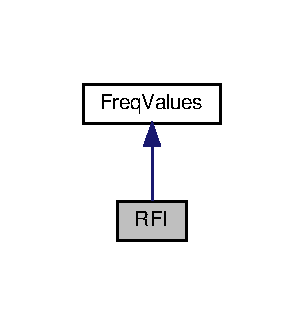
\includegraphics[width=146pt]{structRFI__inherit__graph}
\end{center}
\end{figure}


Collaboration diagram for R\+FI\+:\nopagebreak
\begin{figure}[H]
\begin{center}
\leavevmode
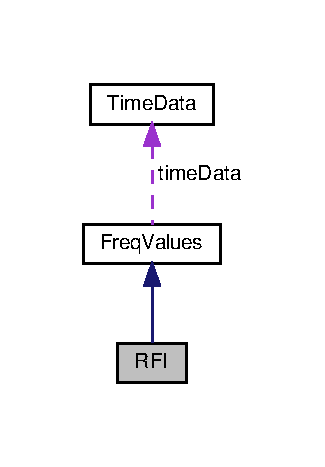
\includegraphics[width=156pt]{structRFI__coll__graph}
\end{center}
\end{figure}
\subsection*{Public Types}
\begin{DoxyCompactItemize}
\item 
\mbox{\Hypertarget{structRFI_a18cfa7d24274bbcd14acc6b513860cb0}\label{structRFI_a18cfa7d24274bbcd14acc6b513860cb0}} 
enum \hyperlink{structRFI_a18cfa7d24274bbcd14acc6b513860cb0}{Thresholds\+Norm} \{ {\bfseries I\+T\+U\+\_\+\+R\+A769\+\_\+2\+\_\+\+V\+L\+BI}, 
{\bfseries S\+K\+A\+\_\+\+M\+O\+D\+E1}, 
{\bfseries S\+K\+A\+\_\+\+M\+O\+D\+E2}
 \}\begin{DoxyCompactList}\small\item\em Enumeration which contains the reference documents (recommendations, protocols, etc.) of harmful \hyperlink{structRFI}{R\+FI} levels (a.\+k.\+a. thresholds)\+: the I\+TU recommendation R\+A.\+769-\/2, S\+KA protocol Mode 1, S\+KA protocol Mode 2. \end{DoxyCompactList}
\end{DoxyCompactItemize}
\subsection*{Public Member Functions}
\begin{DoxyCompactItemize}
\item 
\mbox{\Hypertarget{structRFI_ad0183cf1bc28c3f907e16428a5816e35}\label{structRFI_ad0183cf1bc28c3f907e16428a5816e35}} 
\hyperlink{structRFI_ad0183cf1bc28c3f907e16428a5816e35}{R\+FI} ()
\begin{DoxyCompactList}\small\item\em The default constructor which calls the default constructor of structure {\itshape \hyperlink{structFreqValues}{Freq\+Values}} and set type to \char`\"{}rfi\char`\"{}, azimuth angle to zero, number of bands to zero and set, by default, threshold norm to S\+K\+A\+\_\+\+M\+O\+D\+E1. \end{DoxyCompactList}\item 
\hyperlink{structRFI_a82852dbeab11484c90d4b339f63aefa9}{R\+FI} (const \hyperlink{structRFI}{R\+FI} \&rfi)
\begin{DoxyCompactList}\small\item\em The copy constructor which receives a {\itshape \hyperlink{structRFI}{R\+FI}} object. \end{DoxyCompactList}\item 
\mbox{\Hypertarget{structRFI_a103d0419053a7e323647cdafb3b036e3}\label{structRFI_a103d0419053a7e323647cdafb3b036e3}} 
void \hyperlink{structRFI_a103d0419053a7e323647cdafb3b036e3}{Clear} ()
\begin{DoxyCompactList}\small\item\em The aim of this method is to clean the attributes of this structure. \end{DoxyCompactList}\item 
const \hyperlink{structRFI}{R\+FI} \& \hyperlink{structRFI_a8fcc866a09f2f88a9754e04a1d056104}{operator=} (const \hyperlink{structRFI}{R\+FI} \&another\+R\+FI)
\begin{DoxyCompactList}\small\item\em An overloading of the assignment operator adapted to receive a {\itshape \hyperlink{structRFI}{R\+FI}} object. \end{DoxyCompactList}\end{DoxyCompactItemize}
\subsection*{Public Attributes}
\begin{DoxyCompactItemize}
\item 
\mbox{\Hypertarget{structRFI_aeb10ac61d7897dbaa6971607e56ea244}\label{structRFI_aeb10ac61d7897dbaa6971607e56ea244}} 
float \hyperlink{structRFI_aeb10ac61d7897dbaa6971607e56ea244}{azimuth\+Angle}
\begin{DoxyCompactList}\small\item\em The azimuth angle where this \hyperlink{structRFI}{R\+FI} was detected. \end{DoxyCompactList}\item 
\mbox{\Hypertarget{structRFI_a6c5345dd1141e8bf80b4e1cf32c092de}\label{structRFI_a6c5345dd1141e8bf80b4e1cf32c092de}} 
std\+::string \hyperlink{structRFI_a6c5345dd1141e8bf80b4e1cf32c092de}{polarization}
\begin{DoxyCompactList}\small\item\em The antenna polarization of the sweep where the \hyperlink{structRFI}{R\+FI} was detected. \end{DoxyCompactList}\item 
\mbox{\Hypertarget{structRFI_aefedd07c1a853fb1c8363a0f436d3973}\label{structRFI_aefedd07c1a853fb1c8363a0f436d3973}} 
unsigned int \hyperlink{structRFI_aefedd07c1a853fb1c8363a0f436d3973}{num\+Of\+R\+F\+I\+Bands}
\begin{DoxyCompactList}\small\item\em The number of \hyperlink{structRFI}{R\+FI} bands defined as intervals of continuous data points where it was detected \hyperlink{structRFI}{R\+FI}. \end{DoxyCompactList}\item 
\hyperlink{structRFI_a18cfa7d24274bbcd14acc6b513860cb0}{Thresholds\+Norm} \hyperlink{structRFI_a48905b3dcebf7127bd31315a21a24599}{thresh\+Norm}
\end{DoxyCompactItemize}


\subsection{Detailed Description}
The aim of this structure is to store the data related with the detected RF interference (\hyperlink{structRFI}{R\+FI})\+: frequency, power, azimuth angle, polarization, time, reference norm, etc. 

\subsection{Constructor \& Destructor Documentation}
\mbox{\Hypertarget{structRFI_a82852dbeab11484c90d4b339f63aefa9}\label{structRFI_a82852dbeab11484c90d4b339f63aefa9}} 
\index{R\+FI@{R\+FI}!R\+FI@{R\+FI}}
\index{R\+FI@{R\+FI}!R\+FI@{R\+FI}}
\subsubsection{\texorpdfstring{R\+F\+I()}{RFI()}}
{\footnotesize\ttfamily R\+F\+I\+::\+R\+FI (\begin{DoxyParamCaption}\item[{const \hyperlink{structRFI}{R\+FI} \&}]{rfi }\end{DoxyParamCaption})\hspace{0.3cm}{\ttfamily [inline]}}



The copy constructor which receives a {\itshape \hyperlink{structRFI}{R\+FI}} object. 


\begin{DoxyParams}[1]{Parameters}
\mbox{\tt in}  & {\em rfi} & A {\itshape \hyperlink{structRFI}{R\+FI}} structure given to copy its attributes. \\
\hline
\end{DoxyParams}


\subsection{Member Function Documentation}
\mbox{\Hypertarget{structRFI_a8fcc866a09f2f88a9754e04a1d056104}\label{structRFI_a8fcc866a09f2f88a9754e04a1d056104}} 
\index{R\+FI@{R\+FI}!operator=@{operator=}}
\index{operator=@{operator=}!R\+FI@{R\+FI}}
\subsubsection{\texorpdfstring{operator=()}{operator=()}}
{\footnotesize\ttfamily const \hyperlink{structRFI}{R\+FI}\& R\+F\+I\+::operator= (\begin{DoxyParamCaption}\item[{const \hyperlink{structRFI}{R\+FI} \&}]{another\+R\+FI }\end{DoxyParamCaption})\hspace{0.3cm}{\ttfamily [inline]}}



An overloading of the assignment operator adapted to receive a {\itshape \hyperlink{structRFI}{R\+FI}} object. 


\begin{DoxyParams}[1]{Parameters}
\mbox{\tt in}  & {\em another\+R\+FI} & Another {\itshape \hyperlink{structRFI}{R\+FI}} structure given to copy its attributes. \\
\hline
\end{DoxyParams}


\subsection{Member Data Documentation}
\mbox{\Hypertarget{structRFI_a48905b3dcebf7127bd31315a21a24599}\label{structRFI_a48905b3dcebf7127bd31315a21a24599}} 
\index{R\+FI@{R\+FI}!thresh\+Norm@{thresh\+Norm}}
\index{thresh\+Norm@{thresh\+Norm}!R\+FI@{R\+FI}}
\subsubsection{\texorpdfstring{thresh\+Norm}{threshNorm}}
{\footnotesize\ttfamily \hyperlink{structRFI_a18cfa7d24274bbcd14acc6b513860cb0}{Thresholds\+Norm} R\+F\+I\+::thresh\+Norm}

The norm (recommendation, protocol, etc.) which was used to define the harmful interference levels. 

The documentation for this struct was generated from the following file\+:\begin{DoxyCompactItemize}
\item 
/home/new-\/mauro/eclipse-\/cdt/workspace/\+R\+F\+I\+M\+S\+\_\+\+C\+A\+R\+T/src/\hyperlink{Basics_8h}{Basics.\+h}\end{DoxyCompactItemize}

\hypertarget{structSweep}{}\section{Sweep Struct Reference}
\label{structSweep}\index{Sweep@{Sweep}}


The aim of this structure is to store the data points of a sweep obtained with the spectrum analyzer in a determined azimuth position, with a specific polarization.  




{\ttfamily \#include $<$Basics.\+h$>$}



Inheritance diagram for Sweep\+:\nopagebreak
\begin{figure}[H]
\begin{center}
\leavevmode
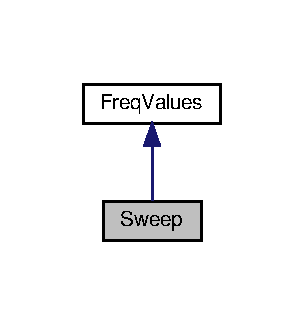
\includegraphics[width=146pt]{structSweep__inherit__graph}
\end{center}
\end{figure}


Collaboration diagram for Sweep\+:\nopagebreak
\begin{figure}[H]
\begin{center}
\leavevmode
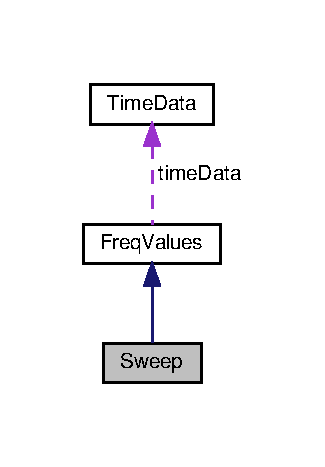
\includegraphics[width=156pt]{structSweep__coll__graph}
\end{center}
\end{figure}
\subsection*{Public Member Functions}
\begin{DoxyCompactItemize}
\item 
\mbox{\Hypertarget{structSweep_a154d8154b44ffd83c26375ca8d688591}\label{structSweep_a154d8154b44ffd83c26375ca8d688591}} 
\hyperlink{structSweep_a154d8154b44ffd83c26375ca8d688591}{Sweep} ()
\begin{DoxyCompactList}\small\item\em The default constructor which calls the default constructor of {\itshape \hyperlink{structFreqValues}{Freq\+Values}} structure and set type to \char`\"{}sweep\char`\"{} and azimuth angle to zero. \end{DoxyCompactList}\item 
\mbox{\Hypertarget{structSweep_ae85ac9f2a48f93e3fc510118c7d67f7f}\label{structSweep_ae85ac9f2a48f93e3fc510118c7d67f7f}} 
\hyperlink{structSweep_ae85ac9f2a48f93e3fc510118c7d67f7f}{Sweep} (const \hyperlink{structFreqValues}{Freq\+Values} \&freq\+Values)
\begin{DoxyCompactList}\small\item\em A copy constructor which receives a {\itshape \hyperlink{structFreqValues}{Freq\+Values}} object. \end{DoxyCompactList}\item 
\mbox{\Hypertarget{structSweep_a0a4e0f72fe9051d35cb29953005463b3}\label{structSweep_a0a4e0f72fe9051d35cb29953005463b3}} 
\hyperlink{structSweep_a0a4e0f72fe9051d35cb29953005463b3}{Sweep} (const \hyperlink{structSweep}{Sweep} \&sweep)
\begin{DoxyCompactList}\small\item\em A copy constructor which receives a {\itshape \hyperlink{structSweep}{Sweep}} object. \end{DoxyCompactList}\item 
\mbox{\Hypertarget{structSweep_aa852ab0cf53dc52ec354649cf6cec31e}\label{structSweep_aa852ab0cf53dc52ec354649cf6cec31e}} 
void \hyperlink{structSweep_aa852ab0cf53dc52ec354649cf6cec31e}{Clear} ()
\begin{DoxyCompactList}\small\item\em The aim of this method is to clean the structure, i.\+e. to delete all data points, set azimuth angle to zero and clean polarization. \end{DoxyCompactList}\item 
\mbox{\Hypertarget{structSweep_ae20eba1adf7d9510a2433ce942b14007}\label{structSweep_ae20eba1adf7d9510a2433ce942b14007}} 
const \hyperlink{structSweep}{Sweep} \& \hyperlink{structSweep_ae20eba1adf7d9510a2433ce942b14007}{operator=} (const \hyperlink{structSweep}{Sweep} \&sweep)
\begin{DoxyCompactList}\small\item\em An overloading of the assignment operator adapted to this structure. \end{DoxyCompactList}\end{DoxyCompactItemize}
\subsection*{Public Attributes}
\begin{DoxyCompactItemize}
\item 
\mbox{\Hypertarget{structSweep_a1400ee785843eba210c37a8f7e24c941}\label{structSweep_a1400ee785843eba210c37a8f7e24c941}} 
float \hyperlink{structSweep_a1400ee785843eba210c37a8f7e24c941}{azimuth\+Angle}
\begin{DoxyCompactList}\small\item\em The azimuth position (or angle) of the antenna when the sweep was captured. \end{DoxyCompactList}\item 
std\+::string \hyperlink{structSweep_a3484c258fdff60e1c109df92a1ba9ae7}{polarization}
\end{DoxyCompactItemize}
\subsection*{Friends}
\begin{DoxyCompactItemize}
\item 
\mbox{\Hypertarget{structSweep_a29420e86f220ed305794c8e560059bbc}\label{structSweep_a29420e86f220ed305794c8e560059bbc}} 
\hyperlink{structSweep}{Sweep} \hyperlink{structSweep_a29420e86f220ed305794c8e560059bbc}{operator-\/} (const \hyperlink{structSweep}{Sweep} \&argument)
\begin{DoxyCompactList}\small\item\em An overloading of the unary operator -\/ which negates a {\itshape \hyperlink{structSweep}{Sweep}} object. \end{DoxyCompactList}\item 
\mbox{\Hypertarget{structSweep_a96391241f10ea728ee36b62f6c35d604}\label{structSweep_a96391241f10ea728ee36b62f6c35d604}} 
\hyperlink{structSweep}{Sweep} \hyperlink{structSweep_a96391241f10ea728ee36b62f6c35d604}{operator+} (const \hyperlink{structSweep}{Sweep} \&lhs, const \hyperlink{structSweep}{Sweep} \&rhs)
\begin{DoxyCompactList}\small\item\em An overloading of operator + which calculates the sum of two objects of structure {\itshape \hyperlink{structSweep}{Sweep}}. \end{DoxyCompactList}\item 
\mbox{\Hypertarget{structSweep_ab372b814f572937b3f0cef31752994b9}\label{structSweep_ab372b814f572937b3f0cef31752994b9}} 
\hyperlink{structSweep}{Sweep} \hyperlink{structSweep_ab372b814f572937b3f0cef31752994b9}{operator+} (const \hyperlink{structSweep}{Sweep} \&lhs, const std\+::vector$<$ float $>$ \&rhs)
\begin{DoxyCompactList}\small\item\em An overloading of operator + which calculates the sum of a {\itshape \hyperlink{structSweep}{Sweep}} object and a {\ttfamily std\+::vector$<$float$>$} container, in that order. \end{DoxyCompactList}\item 
\mbox{\Hypertarget{structSweep_a770d2ac63866693c821c99cbfe2b2c9a}\label{structSweep_a770d2ac63866693c821c99cbfe2b2c9a}} 
\hyperlink{structSweep}{Sweep} \hyperlink{structSweep_a770d2ac63866693c821c99cbfe2b2c9a}{operator+} (const std\+::vector$<$ float $>$ \&lhs, const \hyperlink{structSweep}{Sweep} \&rhs)
\begin{DoxyCompactList}\small\item\em An overloading of operator + which calculates the sum of a {\ttfamily std\+::vector$<$float$>$} container and a {\itshape \hyperlink{structSweep}{Sweep}} object, in that order. \end{DoxyCompactList}\item 
\mbox{\Hypertarget{structSweep_a5d6fad874c778ae77a10b57446a0bd93}\label{structSweep_a5d6fad874c778ae77a10b57446a0bd93}} 
\hyperlink{structSweep}{Sweep} \hyperlink{structSweep_a5d6fad874c778ae77a10b57446a0bd93}{operator+} (const \hyperlink{structSweep}{Sweep} \&lhs, const \hyperlink{structFreqValues}{Freq\+Values} \&rhs)
\begin{DoxyCompactList}\small\item\em An overloading of operator + which calculates the sum of a {\itshape \hyperlink{structSweep}{Sweep}} object and a {\itshape \hyperlink{structFreqValues}{Freq\+Values}} object, in that order. \end{DoxyCompactList}\item 
\mbox{\Hypertarget{structSweep_ae8dce428f848644d0a68cc8309f88ebf}\label{structSweep_ae8dce428f848644d0a68cc8309f88ebf}} 
\hyperlink{structSweep}{Sweep} \hyperlink{structSweep_ae8dce428f848644d0a68cc8309f88ebf}{operator+} (const \hyperlink{structSweep}{Sweep} \&lhs, const float rhs)
\begin{DoxyCompactList}\small\item\em An overloading of operator + which calculates the sum of a {\itshape \hyperlink{structSweep}{Sweep}} object and a {\itshape float} value, in that order. \end{DoxyCompactList}\item 
\mbox{\Hypertarget{structSweep_ac0d73d5e8e3aab8f87c9815588b66821}\label{structSweep_ac0d73d5e8e3aab8f87c9815588b66821}} 
\hyperlink{structSweep}{Sweep} \hyperlink{structSweep_ac0d73d5e8e3aab8f87c9815588b66821}{operator+} (const float lhs, const \hyperlink{structSweep}{Sweep} \&rhs)
\begin{DoxyCompactList}\small\item\em An overloading of operator + which calculates the sum of a {\itshape float} value and a {\itshape \hyperlink{structSweep}{Sweep}} object, in that order. \end{DoxyCompactList}\item 
\mbox{\Hypertarget{structSweep_a8f704b31d015e4d81d25d3fceca1e2f1}\label{structSweep_a8f704b31d015e4d81d25d3fceca1e2f1}} 
\hyperlink{structSweep}{Sweep} \hyperlink{structSweep_a8f704b31d015e4d81d25d3fceca1e2f1}{operator-\/} (const \hyperlink{structSweep}{Sweep} \&lhs, const \hyperlink{structSweep}{Sweep} \&rhs)
\begin{DoxyCompactList}\small\item\em An overloading of operator -\/ which calculates the subtraction of two objects of structure {\itshape \hyperlink{structSweep}{Sweep}}. \end{DoxyCompactList}\item 
\mbox{\Hypertarget{structSweep_a8b2585969a3c379f744b662fb3bea749}\label{structSweep_a8b2585969a3c379f744b662fb3bea749}} 
\hyperlink{structSweep}{Sweep} \hyperlink{structSweep_a8b2585969a3c379f744b662fb3bea749}{operator-\/} (const \hyperlink{structSweep}{Sweep} \&lhs, const std\+::vector$<$ float $>$ \&rhs)
\begin{DoxyCompactList}\small\item\em An overloading of operator -\/ which calculates the subtraction of a {\itshape \hyperlink{structSweep}{Sweep}} object and a {\ttfamily std\+::vector$<$float$>$} container, in that order. \end{DoxyCompactList}\item 
\mbox{\Hypertarget{structSweep_a840a49afd7973b4b3d1020e15c4c9819}\label{structSweep_a840a49afd7973b4b3d1020e15c4c9819}} 
\hyperlink{structSweep}{Sweep} \hyperlink{structSweep_a840a49afd7973b4b3d1020e15c4c9819}{operator-\/} (const std\+::vector$<$ float $>$ \&lhs, const \hyperlink{structSweep}{Sweep} \&rhs)
\begin{DoxyCompactList}\small\item\em An overloading of operator -\/ which calculates the subtraction of a {\ttfamily std\+::vector$<$float$>$} container and a {\itshape \hyperlink{structSweep}{Sweep}} object, in that order. \end{DoxyCompactList}\item 
\mbox{\Hypertarget{structSweep_a124ea929f6dba249bd4d6bf5476ab621}\label{structSweep_a124ea929f6dba249bd4d6bf5476ab621}} 
\hyperlink{structSweep}{Sweep} \hyperlink{structSweep_a124ea929f6dba249bd4d6bf5476ab621}{operator-\/} (const \hyperlink{structSweep}{Sweep} \&lhs, const \hyperlink{structFreqValues}{Freq\+Values} \&rhs)
\begin{DoxyCompactList}\small\item\em An overloading of operator -\/ which calculates the subtraction of a {\itshape \hyperlink{structSweep}{Sweep}} object and a {\itshape \hyperlink{structFreqValues}{Freq\+Values}} object, in that order. \end{DoxyCompactList}\item 
\mbox{\Hypertarget{structSweep_a4739da92a36e5f8f17b0be140dd327f6}\label{structSweep_a4739da92a36e5f8f17b0be140dd327f6}} 
\hyperlink{structSweep}{Sweep} \hyperlink{structSweep_a4739da92a36e5f8f17b0be140dd327f6}{operator$\ast$} (const \hyperlink{structSweep}{Sweep} \&lhs, const \hyperlink{structSweep}{Sweep} \&rhs)
\begin{DoxyCompactList}\small\item\em An overloading of operator $\ast$ which multiplies two objects of structure {\itshape \hyperlink{structSweep}{Sweep}}. \end{DoxyCompactList}\item 
\mbox{\Hypertarget{structSweep_a12c1f3e5e4869781ca7d90a50f334606}\label{structSweep_a12c1f3e5e4869781ca7d90a50f334606}} 
\hyperlink{structSweep}{Sweep} \hyperlink{structSweep_a12c1f3e5e4869781ca7d90a50f334606}{operator$\ast$} (const \hyperlink{structSweep}{Sweep} \&lhs, const float rhs)
\begin{DoxyCompactList}\small\item\em An overloading of operator $\ast$ which multiplies a {\itshape \hyperlink{structSweep}{Sweep}} object and a {\itshape float} value, in that order. \end{DoxyCompactList}\item 
\mbox{\Hypertarget{structSweep_ad4aac4ab6e7ea49d5bc9ebfa83eb07be}\label{structSweep_ad4aac4ab6e7ea49d5bc9ebfa83eb07be}} 
\hyperlink{structSweep}{Sweep} \hyperlink{structSweep_ad4aac4ab6e7ea49d5bc9ebfa83eb07be}{operator$\ast$} (const float lhs, const \hyperlink{structSweep}{Sweep} \&rhs)
\begin{DoxyCompactList}\small\item\em An overloading of operator $\ast$ which multiplies a {\itshape float} value and a {\itshape \hyperlink{structSweep}{Sweep}} object, in that order. \end{DoxyCompactList}\item 
\mbox{\Hypertarget{structSweep_a3e230f15cb1119940203a1a452676b74}\label{structSweep_a3e230f15cb1119940203a1a452676b74}} 
\hyperlink{structSweep}{Sweep} \hyperlink{structSweep_a3e230f15cb1119940203a1a452676b74}{operator/} (const \hyperlink{structSweep}{Sweep} \&lhs, const \hyperlink{structSweep}{Sweep} \&rhs)
\begin{DoxyCompactList}\small\item\em An overloading of operator / which calculates the division between two objects of structure {\itshape \hyperlink{structSweep}{Sweep}}. \end{DoxyCompactList}\item 
\mbox{\Hypertarget{structSweep_a73694ded6e7ba41c367ca5f0934cbc2c}\label{structSweep_a73694ded6e7ba41c367ca5f0934cbc2c}} 
\hyperlink{structSweep}{Sweep} \hyperlink{structSweep_a73694ded6e7ba41c367ca5f0934cbc2c}{operator/} (const \hyperlink{structSweep}{Sweep} \&lhs, const float rhs)
\begin{DoxyCompactList}\small\item\em An overloading of operator / which calculates the division between a {\itshape \hyperlink{structSweep}{Sweep}} object and a {\itshape float} value, in that order. \end{DoxyCompactList}\item 
\mbox{\Hypertarget{structSweep_abe3c133bf246f7faebcfda286c5e1448}\label{structSweep_abe3c133bf246f7faebcfda286c5e1448}} 
\hyperlink{structSweep}{Sweep} \hyperlink{structSweep_abe3c133bf246f7faebcfda286c5e1448}{operator/} (const float lhs, const \hyperlink{structSweep}{Sweep} \&rhs)
\begin{DoxyCompactList}\small\item\em An overloading of operator / which calculates the division between a {\itshape float} value and a {\itshape \hyperlink{structSweep}{Sweep}} object, in that order. \end{DoxyCompactList}\item 
\mbox{\Hypertarget{structSweep_a37df38f37b1cf6a6bfb18f44b706d308}\label{structSweep_a37df38f37b1cf6a6bfb18f44b706d308}} 
\hyperlink{structSweep}{Sweep} \hyperlink{structSweep_a37df38f37b1cf6a6bfb18f44b706d308}{log10} (const \hyperlink{structSweep}{Sweep} \&argument)
\begin{DoxyCompactList}\small\item\em An overloading of function {\ttfamily \hyperlink{structSweep_a37df38f37b1cf6a6bfb18f44b706d308}{log10()}} adapted to receive an argument of type {\itshape \hyperlink{structSweep}{Sweep}}. \end{DoxyCompactList}\item 
\mbox{\Hypertarget{structSweep_a09ee88cfc9b28e6ec344eea1a2817ea9}\label{structSweep_a09ee88cfc9b28e6ec344eea1a2817ea9}} 
\hyperlink{structSweep}{Sweep} \hyperlink{structSweep_a09ee88cfc9b28e6ec344eea1a2817ea9}{pow} (const \hyperlink{structSweep}{Sweep} \&base, const float exponent)
\begin{DoxyCompactList}\small\item\em An overloading of function {\ttfamily \hyperlink{structSweep_a09ee88cfc9b28e6ec344eea1a2817ea9}{pow()}} adapted to receive an argument of type {\itshape \hyperlink{structSweep}{Sweep}} as base and an argument of type {\itshape float} as exponent. \end{DoxyCompactList}\item 
\mbox{\Hypertarget{structSweep_a879ae44efd2611562d05b90b24099e70}\label{structSweep_a879ae44efd2611562d05b90b24099e70}} 
\hyperlink{structSweep}{Sweep} \hyperlink{structSweep_a879ae44efd2611562d05b90b24099e70}{pow} (const float base, const \hyperlink{structSweep}{Sweep} \&exponent)
\begin{DoxyCompactList}\small\item\em An overloading of function {\ttfamily \hyperlink{structSweep_a09ee88cfc9b28e6ec344eea1a2817ea9}{pow()}} adapted to receive an argument of type {\itshape float} as base and an argument of type {\itshape \hyperlink{structSweep}{Sweep}} as exponent. \end{DoxyCompactList}\end{DoxyCompactItemize}


\subsection{Detailed Description}
The aim of this structure is to store the data points of a sweep obtained with the spectrum analyzer in a determined azimuth position, with a specific polarization. 

\subsection{Member Data Documentation}
\mbox{\Hypertarget{structSweep_a3484c258fdff60e1c109df92a1ba9ae7}\label{structSweep_a3484c258fdff60e1c109df92a1ba9ae7}} 
\index{Sweep@{Sweep}!polarization@{polarization}}
\index{polarization@{polarization}!Sweep@{Sweep}}
\subsubsection{\texorpdfstring{polarization}{polarization}}
{\footnotesize\ttfamily std\+::string Sweep\+::polarization}

The antenna polarization when the sweep was captured. 

The documentation for this struct was generated from the following file\+:\begin{DoxyCompactItemize}
\item 
\hyperlink{Basics_8h}{Basics.\+h}\end{DoxyCompactItemize}

\hypertarget{structTimeData}{}\section{Time\+Data Struct Reference}
\label{structTimeData}\index{Time\+Data@{Time\+Data}}


This structure is intended to store data related to {\itshape date} and {\itshape time} and to perform some operations with that data.  




{\ttfamily \#include $<$Basics.\+h$>$}

\subsection*{Public Member Functions}
\begin{DoxyCompactItemize}
\item 
\mbox{\Hypertarget{structTimeData_a4be51d0cd0dce3b91ce449b6c995a9e9}\label{structTimeData_a4be51d0cd0dce3b91ce449b6c995a9e9}} 
\hyperlink{structTimeData_a4be51d0cd0dce3b91ce449b6c995a9e9}{Time\+Data} ()
\begin{DoxyCompactList}\small\item\em The class\textquotesingle{} constructor which clear all attributes, i.\+e. set date and time as 00-\/00-\/00\+T00\+:00\+:00. \end{DoxyCompactList}\item 
\mbox{\Hypertarget{structTimeData_af0454b54d768d6b21267b3692dae4d3d}\label{structTimeData_af0454b54d768d6b21267b3692dae4d3d}} 
\hyperlink{structTimeData_af0454b54d768d6b21267b3692dae4d3d}{Time\+Data} (const \hyperlink{structTimeData}{Time\+Data} \&time\+Data)
\begin{DoxyCompactList}\small\item\em The class\textquotesingle{} copy constructor. \end{DoxyCompactList}\item 
\mbox{\Hypertarget{structTimeData_a78640fbf87e59255e08836b6779ec5c0}\label{structTimeData_a78640fbf87e59255e08836b6779ec5c0}} 
std\+::string \hyperlink{structTimeData_a78640fbf87e59255e08836b6779ec5c0}{Get\+Date} () const
\begin{DoxyCompactList}\small\item\em A method to get the date as a {\ttfamily std\+::string} \end{DoxyCompactList}\item 
\mbox{\Hypertarget{structTimeData_a6810621b9bd2289b697a7cd7b1799515}\label{structTimeData_a6810621b9bd2289b697a7cd7b1799515}} 
std\+::string \hyperlink{structTimeData_a6810621b9bd2289b697a7cd7b1799515}{Get\+Time} () const
\begin{DoxyCompactList}\small\item\em A method to get the time as a {\ttfamily std\+::string} \end{DoxyCompactList}\item 
\mbox{\Hypertarget{structTimeData_a06956ece691807dc69e4fe6add2bd423}\label{structTimeData_a06956ece691807dc69e4fe6add2bd423}} 
std\+::string \hyperlink{structTimeData_a06956ece691807dc69e4fe6add2bd423}{Get\+Timestamp} () const
\begin{DoxyCompactList}\small\item\em A method to get a timestamp as a {\ttfamily std\+::string} with the format D\+D-\/\+M\+M-\/\+Y\+Y\+Y\+Y\+T\+HH\+:MM\+:SS. \end{DoxyCompactList}\item 
\mbox{\Hypertarget{structTimeData_ac4a84f214fbaeaac5fa77df2c68bad79}\label{structTimeData_ac4a84f214fbaeaac5fa77df2c68bad79}} 
void \hyperlink{structTimeData_ac4a84f214fbaeaac5fa77df2c68bad79}{Set\+Date} (const std\+::string \&date)
\begin{DoxyCompactList}\small\item\em This method is intended to set just the date. \end{DoxyCompactList}\item 
\mbox{\Hypertarget{structTimeData_a79c359b6aa1d5362065105d0e6b2f657}\label{structTimeData_a79c359b6aa1d5362065105d0e6b2f657}} 
void \hyperlink{structTimeData_a79c359b6aa1d5362065105d0e6b2f657}{Set\+Time} (const std\+::string \&time)
\begin{DoxyCompactList}\small\item\em This method is intended to set just the time. \end{DoxyCompactList}\item 
\mbox{\Hypertarget{structTimeData_a753d18acb1fdebbde3e910e2462b4073}\label{structTimeData_a753d18acb1fdebbde3e910e2462b4073}} 
void \hyperlink{structTimeData_a753d18acb1fdebbde3e910e2462b4073}{Set\+Timestamp} (const std\+::string \&timestamp)
\begin{DoxyCompactList}\small\item\em This method is intended to modify all attributes, giving these as a timestamp. \end{DoxyCompactList}\item 
\mbox{\Hypertarget{structTimeData_ad204062485d50c24aad1d4b41a582bd8}\label{structTimeData_ad204062485d50c24aad1d4b41a582bd8}} 
void \hyperlink{structTimeData_ad204062485d50c24aad1d4b41a582bd8}{Turn\+Back\+Days} (const unsigned int days)
\begin{DoxyCompactList}\small\item\em This method allows to turn a time point back a specified number of days. \end{DoxyCompactList}\item 
\mbox{\Hypertarget{structTimeData_a43ba78733adf4369e4c8c89db1819772}\label{structTimeData_a43ba78733adf4369e4c8c89db1819772}} 
const \hyperlink{structTimeData}{Time\+Data} \& \hyperlink{structTimeData_a43ba78733adf4369e4c8c89db1819772}{operator=} (const \hyperlink{structTimeData}{Time\+Data} \&another\+Time\+Data)
\begin{DoxyCompactList}\small\item\em An overloading of the assignmetn operator. \end{DoxyCompactList}\item 
\mbox{\Hypertarget{structTimeData_af1071330f0fadc98a5e08d41a8436907}\label{structTimeData_af1071330f0fadc98a5e08d41a8436907}} 
void \hyperlink{structTimeData_af1071330f0fadc98a5e08d41a8436907}{Clear} ()
\begin{DoxyCompactList}\small\item\em A method to clear all attributes, i.\+e. it set the object as 00-\/00-\/00\+T00\+:00\+:00. \end{DoxyCompactList}\end{DoxyCompactItemize}
\subsection*{Public Attributes}
\begin{DoxyCompactItemize}
\item 
\mbox{\Hypertarget{structTimeData_a457ba435747cdc51aa3c9213dc75e916}\label{structTimeData_a457ba435747cdc51aa3c9213dc75e916}} 
unsigned int \hyperlink{structTimeData_a457ba435747cdc51aa3c9213dc75e916}{year}
\begin{DoxyCompactList}\small\item\em This variable stores the year, taking into account the estimated birth of Jesus. \end{DoxyCompactList}\item 
\mbox{\Hypertarget{structTimeData_a54ec81ff233394814cb837c41cd3ea0b}\label{structTimeData_a54ec81ff233394814cb837c41cd3ea0b}} 
unsigned int \hyperlink{structTimeData_a54ec81ff233394814cb837c41cd3ea0b}{month}
\begin{DoxyCompactList}\small\item\em This variable stores the month as a number that can be between 1 and 12. \end{DoxyCompactList}\item 
\mbox{\Hypertarget{structTimeData_aee725dc9551cd482534c155a168b3d60}\label{structTimeData_aee725dc9551cd482534c155a168b3d60}} 
unsigned int \hyperlink{structTimeData_aee725dc9551cd482534c155a168b3d60}{day}
\begin{DoxyCompactList}\small\item\em This variable stores the day as a number that can be between 1 and 31, taking into account the corresponding month. \end{DoxyCompactList}\item 
\mbox{\Hypertarget{structTimeData_a989207381ecc5a4c744bd06bf1091c63}\label{structTimeData_a989207381ecc5a4c744bd06bf1091c63}} 
unsigned int \hyperlink{structTimeData_a989207381ecc5a4c744bd06bf1091c63}{hour}
\begin{DoxyCompactList}\small\item\em This variable stores the hours as a number that can be between 0 and 23. \end{DoxyCompactList}\item 
\mbox{\Hypertarget{structTimeData_ac22938d020a988bebae2493b118b9df2}\label{structTimeData_ac22938d020a988bebae2493b118b9df2}} 
unsigned int \hyperlink{structTimeData_ac22938d020a988bebae2493b118b9df2}{minute}
\begin{DoxyCompactList}\small\item\em This variable stores the minutes as a number that can be between 0 and 59. \end{DoxyCompactList}\item 
\mbox{\Hypertarget{structTimeData_ac17cd0725bea21f3be277d2c9a00e3d8}\label{structTimeData_ac17cd0725bea21f3be277d2c9a00e3d8}} 
unsigned int \hyperlink{structTimeData_ac17cd0725bea21f3be277d2c9a00e3d8}{second}
\begin{DoxyCompactList}\small\item\em This variable stores the seconds as a number that can be between 0 and 59. \end{DoxyCompactList}\end{DoxyCompactItemize}
\subsection*{Friends}
\begin{DoxyCompactItemize}
\item 
\mbox{\Hypertarget{structTimeData_a05ed1f021fd859fd0507d8ec74de5afd}\label{structTimeData_a05ed1f021fd859fd0507d8ec74de5afd}} 
bool \hyperlink{structTimeData_a05ed1f021fd859fd0507d8ec74de5afd}{operator$<$} (const \hyperlink{structTimeData}{Time\+Data} \&lhs, const \hyperlink{structTimeData}{Time\+Data} \&rhs)
\begin{DoxyCompactList}\small\item\em An overloading of the operator $<$ to compare two \hyperlink{structTimeData}{Time\+Data} objects as the first one lesser than the second one. \end{DoxyCompactList}\item 
\mbox{\Hypertarget{structTimeData_a6ba5c50a9564dae90072889e68cc8a42}\label{structTimeData_a6ba5c50a9564dae90072889e68cc8a42}} 
bool \hyperlink{structTimeData_a6ba5c50a9564dae90072889e68cc8a42}{operator$>$} (const \hyperlink{structTimeData}{Time\+Data} \&lhs, const \hyperlink{structTimeData}{Time\+Data} \&rhs)
\begin{DoxyCompactList}\small\item\em An overloading of the operator $>$ to compare two \hyperlink{structTimeData}{Time\+Data} objects as the first one bigger than the second one. \end{DoxyCompactList}\item 
\mbox{\Hypertarget{structTimeData_a77e7e3db1d21909c98eb40309a3ac989}\label{structTimeData_a77e7e3db1d21909c98eb40309a3ac989}} 
bool \hyperlink{structTimeData_a77e7e3db1d21909c98eb40309a3ac989}{operator==} (const \hyperlink{structTimeData}{Time\+Data} \&lhs, const \hyperlink{structTimeData}{Time\+Data} \&rhs)
\begin{DoxyCompactList}\small\item\em An overloading of the operator == to compare two \hyperlink{structTimeData}{Time\+Data} objects as equal. \end{DoxyCompactList}\end{DoxyCompactItemize}


\subsection{Detailed Description}
This structure is intended to store data related to {\itshape date} and {\itshape time} and to perform some operations with that data. 

This structure can store time data (hour, minute and second) and date data (year, month and date) which are obtained from a G\+PS receiver. It can offer just the date as a string, or just the time as a string or even can build a {\itshape timestamp} with a specific format\+: D\+D-\/\+M\+M-\/\+Y\+Y\+Y\+Y\+T\+HH\+:MM\+:SS. Also it can take a date and time and turn that back a specific number of days taking into account the {\itshape gregorian} calendar. An object of this class can even be compared as equal to, less than or bigger than another object of the same class. 

The documentation for this struct was generated from the following file\+:\begin{DoxyCompactItemize}
\item 
\hyperlink{Basics_8h}{Basics.\+h}\end{DoxyCompactItemize}

\chapter{File Documentation}
\hypertarget{Basics_8cpp}{}\section{/home/new-\/mauro/eclipse-\/cdt/workspace/\+R\+F\+I\+M\+S\+\_\+\+C\+A\+R\+T/src/\+Basics.cpp File Reference}
\label{Basics_8cpp}\index{/home/new-\/mauro/eclipse-\/cdt/workspace/\+R\+F\+I\+M\+S\+\_\+\+C\+A\+R\+T/src/\+Basics.\+cpp@{/home/new-\/mauro/eclipse-\/cdt/workspace/\+R\+F\+I\+M\+S\+\_\+\+C\+A\+R\+T/src/\+Basics.\+cpp}}


This file contains the definitions of the functions and classes\textquotesingle{} methods which have been declared in file \hyperlink{Basics_8h}{Basics.\+h}.  


{\ttfamily \#include \char`\"{}Basics.\+h\char`\"{}}\newline
Include dependency graph for Basics.\+cpp\+:\nopagebreak
\begin{figure}[H]
\begin{center}
\leavevmode
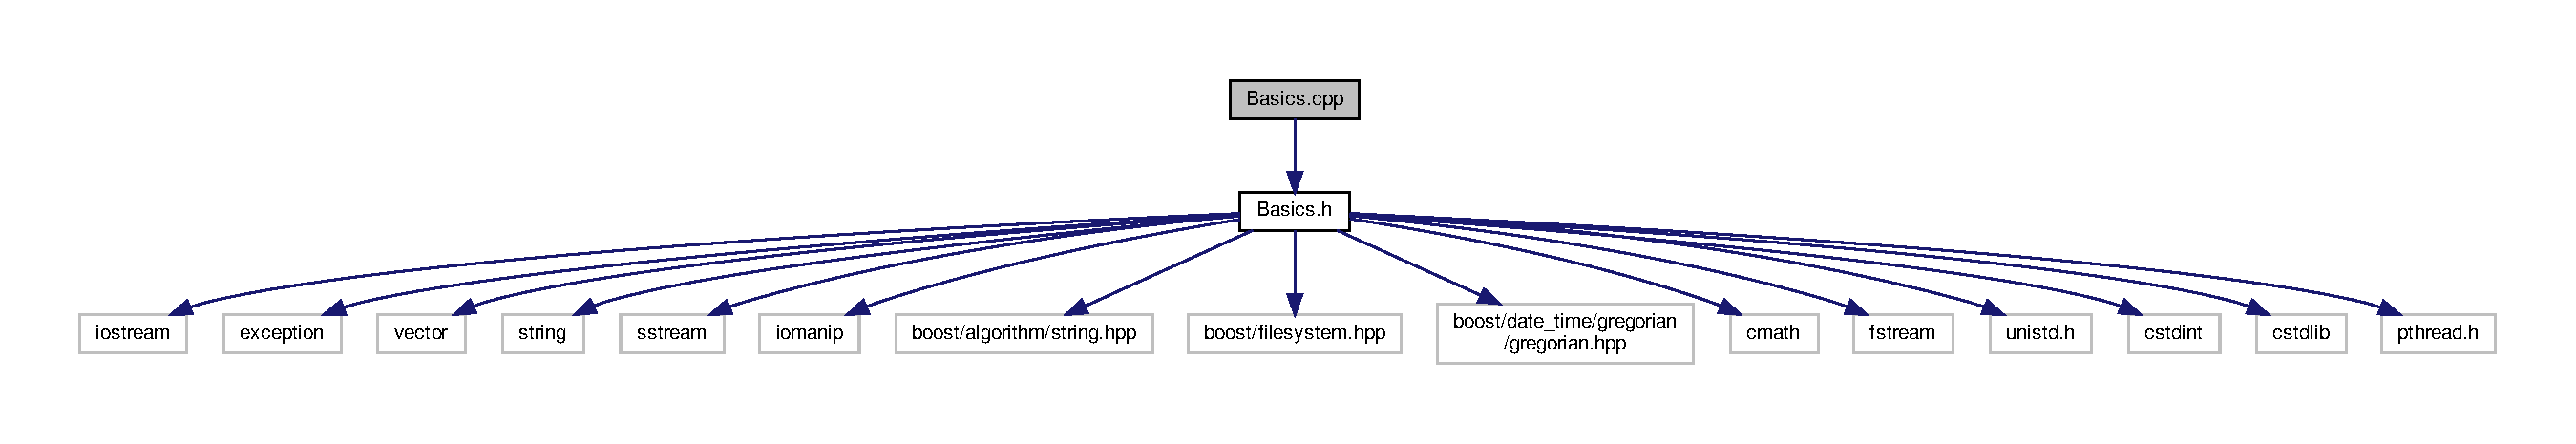
\includegraphics[width=350pt]{Basics_8cpp__incl}
\end{center}
\end{figure}
\subsection*{Functions}
\begin{DoxyCompactItemize}
\item 
bool \hyperlink{Basics_8cpp_ab0cf00620947abc90fbfe36db36f8fc7}{approximately\+Equal} (float a, float b)
\begin{DoxyCompactList}\small\item\em Function intended to compare floating-\/point numbers as approximately equal, taking into account the floating-\/point rounding errors. \end{DoxyCompactList}\item 
bool \hyperlink{Basics_8cpp_adee734e43e4a9a5f4b9f610ccdd3f8e0}{approximately\+Equal} (std\+::vector$<$ float $>$ vectorA, std\+::vector$<$ float $>$ vectorB)
\begin{DoxyCompactList}\small\item\em Function intended to compare {\ttfamily std\+::vector$<$float$>$} containers as approximately equal, taking into account the floating-\/point rounding errors. \end{DoxyCompactList}\item 
\mbox{\Hypertarget{Basics_8cpp_abe6b1466ff5e3b09c33ca5dc9fc81c5a}\label{Basics_8cpp_abe6b1466ff5e3b09c33ca5dc9fc81c5a}} 
void \hyperlink{Basics_8cpp_abe6b1466ff5e3b09c33ca5dc9fc81c5a}{Wait\+For\+Key} ()
\begin{DoxyCompactList}\small\item\em This function stop the execution up to any key is pressed by the user and it was used for debugging purpose. \end{DoxyCompactList}\item 
std\+::vector$<$ float $>$ \hyperlink{Basics_8cpp_ac744212c600f3f610807ec4add576822}{operator-\/} (const std\+::vector$<$ float $>$ \&\hyperlink{Spectran_8h_a16fa8eb91a19fde7a399d85c521f63fd}{vect})
\begin{DoxyCompactList}\small\item\em An overloading of unary operator -\/ which negates the elements of a {\ttfamily std\+::vector$<$float$>$} container. \end{DoxyCompactList}\item 
\mbox{\Hypertarget{Basics_8cpp_adb434b11769fc3a9acd409f2fe534395}\label{Basics_8cpp_adb434b11769fc3a9acd409f2fe534395}} 
void \hyperlink{Basics_8cpp_adb434b11769fc3a9acd409f2fe534395}{Initialize\+G\+P\+IO} ()
\begin{DoxyCompactList}\small\item\em This function initializes all G\+P\+IO pins which are used for the input and output signals, in the way it is described in structure {\itshape pi\+Pins}. \end{DoxyCompactList}\item 
\mbox{\Hypertarget{Basics_8cpp_a37d643c013d8e020715ec625553673e7}\label{Basics_8cpp_a37d643c013d8e020715ec625553673e7}} 
void \hyperlink{Basics_8cpp_a37d643c013d8e020715ec625553673e7}{Turn\+Off\+Leds} ()
\begin{DoxyCompactList}\small\item\em The aim of this function is to turn all L\+E\+Ds off. \end{DoxyCompactList}\item 
void \hyperlink{Basics_8cpp_a2f7418278fcdac50f5c6a73744f8013c}{Turn\+On\+Front\+End} ()
\begin{DoxyCompactList}\small\item\em The aim of this function is to turn on the RF front-\/end elements in a sequential manner, from the spectrum analyzer to the antenna.. \end{DoxyCompactList}\item 
void \hyperlink{Basics_8cpp_a5ffe8b7dfe9c6702ed65b2b8b47bc3e1}{Turn\+Off\+Front\+End} ()
\begin{DoxyCompactList}\small\item\em The aim of this function is to turn off the RF front-\/end elements in a sequential manner, from the antenna to the spectrum analyzer. \end{DoxyCompactList}\item 
\mbox{\Hypertarget{Basics_8cpp_ae964ff8411b4fdcaf65cb5529aea4bef}\label{Basics_8cpp_ae964ff8411b4fdcaf65cb5529aea4bef}} 
void \hyperlink{Basics_8cpp_ae964ff8411b4fdcaf65cb5529aea4bef}{Print\+Help} ()
\begin{DoxyCompactList}\small\item\em This function prints in the {\ttfamily stdout} a message whit a software description and the descriptions of its arguments. \end{DoxyCompactList}\item 
bool \hyperlink{Basics_8cpp_abab505eef94a08a9092f916c62637071}{Process\+Main\+Arguments} (int argc, char $\ast$argv\mbox{[}$\,$\mbox{]})
\begin{DoxyCompactList}\small\item\em This function process the software\textquotesingle{}s arguments, which define the behavior of this one. \end{DoxyCompactList}\end{DoxyCompactItemize}


\subsection{Detailed Description}
This file contains the definitions of the functions and classes\textquotesingle{} methods which have been declared in file \hyperlink{Basics_8h}{Basics.\+h}. 

\begin{DoxyAuthor}{Author}
Mauro Diamantino 
\end{DoxyAuthor}


\subsection{Function Documentation}
\mbox{\Hypertarget{Basics_8cpp_ab0cf00620947abc90fbfe36db36f8fc7}\label{Basics_8cpp_ab0cf00620947abc90fbfe36db36f8fc7}} 
\index{Basics.\+cpp@{Basics.\+cpp}!approximately\+Equal@{approximately\+Equal}}
\index{approximately\+Equal@{approximately\+Equal}!Basics.\+cpp@{Basics.\+cpp}}
\subsubsection{\texorpdfstring{approximately\+Equal()}{approximatelyEqual()}\hspace{0.1cm}{\footnotesize\ttfamily [1/2]}}
{\footnotesize\ttfamily bool approximately\+Equal (\begin{DoxyParamCaption}\item[{float}]{a,  }\item[{float}]{b }\end{DoxyParamCaption})}



Function intended to compare floating-\/point numbers as approximately equal, taking into account the floating-\/point rounding errors. 

This function was copied from this \href{https://www.learncpp.com/cpp-tutorial/35-relational-operators-comparisons/}{\tt link}, but it was modified. It is based in the Knuth’s algorithm but it uses two epsilons, an absolute epsilon (A\+B\+S\+\_\+\+E\+P\+S\+I\+L\+ON) which is very small and is intended to compare near-\/zero floating-\/point numbers and a relative epsilon (R\+E\+L\+\_\+\+E\+P\+S\+I\+L\+ON, which is a percentage of the biggest operand) to compare the rest of the floating-\/point numbers. The function returns true if the difference between a and b is less than A\+B\+S\+\_\+\+E\+P\+S\+I\+L\+ON, or within R\+E\+L\+\_\+\+E\+P\+S\+I\+L\+ON percent of the larger of a and b. 
\begin{DoxyParams}[1]{Parameters}
\mbox{\tt in}  & {\em a} & The left-\/hand side argument. \\
\hline
\mbox{\tt in}  & {\em b} & The right-\/hand side argument. \\
\hline
\end{DoxyParams}
\mbox{\Hypertarget{Basics_8cpp_adee734e43e4a9a5f4b9f610ccdd3f8e0}\label{Basics_8cpp_adee734e43e4a9a5f4b9f610ccdd3f8e0}} 
\index{Basics.\+cpp@{Basics.\+cpp}!approximately\+Equal@{approximately\+Equal}}
\index{approximately\+Equal@{approximately\+Equal}!Basics.\+cpp@{Basics.\+cpp}}
\subsubsection{\texorpdfstring{approximately\+Equal()}{approximatelyEqual()}\hspace{0.1cm}{\footnotesize\ttfamily [2/2]}}
{\footnotesize\ttfamily bool approximately\+Equal (\begin{DoxyParamCaption}\item[{std\+::vector$<$ float $>$}]{vectorA,  }\item[{std\+::vector$<$ float $>$}]{vectorB }\end{DoxyParamCaption})}



Function intended to compare {\ttfamily std\+::vector$<$float$>$} containers as approximately equal, taking into account the floating-\/point rounding errors. 

This function is based on the function presented in this \href{https://www.learncpp.com/cpp-tutorial/35-relational-operators-comparisons/}{\tt link}.

It is based in the Knuth’s algorithm but it uses two epsilons, an absolute epsilon (A\+B\+S\+\_\+\+E\+P\+S\+I\+L\+ON) which is very small and is intended to compare near-\/zero floating-\/point numbers and a relative epsilon (R\+E\+L\+\_\+\+E\+P\+S\+I\+L\+ON, which is a percentage of the biggest operand) to compare the rest of the floating-\/point numbers. The function returns true if the difference between a and b is less than A\+B\+S\+\_\+\+E\+P\+S\+I\+L\+ON, or within R\+E\+L\+\_\+\+E\+P\+S\+I\+L\+ON percent of the larger of a and b. 
\begin{DoxyParams}[1]{Parameters}
\mbox{\tt in}  & {\em vectorA} & The left-\/hand side argument. \\
\hline
\mbox{\tt in}  & {\em vectorB} & The right-\/hand side argument. \\
\hline
\end{DoxyParams}
\mbox{\Hypertarget{Basics_8cpp_ac744212c600f3f610807ec4add576822}\label{Basics_8cpp_ac744212c600f3f610807ec4add576822}} 
\index{Basics.\+cpp@{Basics.\+cpp}!operator-\/@{operator-\/}}
\index{operator-\/@{operator-\/}!Basics.\+cpp@{Basics.\+cpp}}
\subsubsection{\texorpdfstring{operator-\/()}{operator-()}}
{\footnotesize\ttfamily std\+::vector$<$float$>$ operator-\/ (\begin{DoxyParamCaption}\item[{const std\+::vector$<$ float $>$ \&}]{vect }\end{DoxyParamCaption})}



An overloading of unary operator -\/ which negates the elements of a {\ttfamily std\+::vector$<$float$>$} container. 


\begin{DoxyParams}[1]{Parameters}
\mbox{\tt in}  & {\em vect} & A {\ttfamily std\+::vector$<$float$>$} container which must be negated. \\
\hline
\end{DoxyParams}
\mbox{\Hypertarget{Basics_8cpp_abab505eef94a08a9092f916c62637071}\label{Basics_8cpp_abab505eef94a08a9092f916c62637071}} 
\index{Basics.\+cpp@{Basics.\+cpp}!Process\+Main\+Arguments@{Process\+Main\+Arguments}}
\index{Process\+Main\+Arguments@{Process\+Main\+Arguments}!Basics.\+cpp@{Basics.\+cpp}}
\subsubsection{\texorpdfstring{Process\+Main\+Arguments()}{ProcessMainArguments()}}
{\footnotesize\ttfamily bool Process\+Main\+Arguments (\begin{DoxyParamCaption}\item[{int}]{argc,  }\item[{char $\ast$}]{argv\mbox{[}$\,$\mbox{]} }\end{DoxyParamCaption})}



This function process the software\textquotesingle{}s arguments, which define the behavior of this one. 

This function determines the values of the behavior flags (flag\+Cal\+Enabled, flag\+Plot, flag\+R\+FI, etc.) taking into account the arguments that were received and its values. The function returns a {\ttfamily true} value if the arguments were processed correctly and a {\ttfamily false} value if there was an argument which could not be recognized, and in that case it presents a message, in the {\ttfamily stdout}, explaining the correct use of the software arguments. 
\begin{DoxyParams}[1]{Parameters}
\mbox{\tt in}  & {\em argc} & The number of arguments that were received by the software. \\
\hline
\mbox{\tt in}  & {\em argv} & An array of C strings ({\ttfamily char$\ast$}) where each one is a software\textquotesingle{}s argument. \\
\hline
\end{DoxyParams}
\mbox{\Hypertarget{Basics_8cpp_a5ffe8b7dfe9c6702ed65b2b8b47bc3e1}\label{Basics_8cpp_a5ffe8b7dfe9c6702ed65b2b8b47bc3e1}} 
\index{Basics.\+cpp@{Basics.\+cpp}!Turn\+Off\+Front\+End@{Turn\+Off\+Front\+End}}
\index{Turn\+Off\+Front\+End@{Turn\+Off\+Front\+End}!Basics.\+cpp@{Basics.\+cpp}}
\subsubsection{\texorpdfstring{Turn\+Off\+Front\+End()}{TurnOffFrontEnd()}}
{\footnotesize\ttfamily void Turn\+Off\+Front\+End (\begin{DoxyParamCaption}{ }\end{DoxyParamCaption})}



The aim of this function is to turn off the RF front-\/end elements in a sequential manner, from the antenna to the spectrum analyzer. 

To turn off the RF front-\/end elements sequentially, this function begins ensuring the noise source is turned off, then it switches the input to that device, it waits 1 second, it turns the L\+N\+As off, it waits again 1 second and, finally, it turns the spectrum analyzer off. \mbox{\Hypertarget{Basics_8cpp_a2f7418278fcdac50f5c6a73744f8013c}\label{Basics_8cpp_a2f7418278fcdac50f5c6a73744f8013c}} 
\index{Basics.\+cpp@{Basics.\+cpp}!Turn\+On\+Front\+End@{Turn\+On\+Front\+End}}
\index{Turn\+On\+Front\+End@{Turn\+On\+Front\+End}!Basics.\+cpp@{Basics.\+cpp}}
\subsubsection{\texorpdfstring{Turn\+On\+Front\+End()}{TurnOnFrontEnd()}}
{\footnotesize\ttfamily void Turn\+On\+Front\+End (\begin{DoxyParamCaption}{ }\end{DoxyParamCaption})}



The aim of this function is to turn on the RF front-\/end elements in a sequential manner, from the spectrum analyzer to the antenna.. 

To turn on the RF front-\/end elements in a sequential manner, first, this function turns the spectrum analyzer on, then it waits 5 seconds, it turns the L\+N\+As on, it waits again but this time just 1 second and, finally, it switches the input to the antenna. 
\hypertarget{Basics_8h}{}\section{/home/new-\/mauro/eclipse-\/cdt/workspace/\+R\+F\+I\+M\+S\+\_\+\+C\+A\+R\+T/src/\+Basics.h File Reference}
\label{Basics_8h}\index{/home/new-\/mauro/eclipse-\/cdt/workspace/\+R\+F\+I\+M\+S\+\_\+\+C\+A\+R\+T/src/\+Basics.\+h@{/home/new-\/mauro/eclipse-\/cdt/workspace/\+R\+F\+I\+M\+S\+\_\+\+C\+A\+R\+T/src/\+Basics.\+h}}


This header file contains the declarations of the most basic and global entities which are used by many others entities.  


{\ttfamily \#include $<$iostream$>$}\newline
{\ttfamily \#include $<$exception$>$}\newline
{\ttfamily \#include $<$vector$>$}\newline
{\ttfamily \#include $<$string$>$}\newline
{\ttfamily \#include $<$sstream$>$}\newline
{\ttfamily \#include $<$iomanip$>$}\newline
{\ttfamily \#include $<$boost/algorithm/string.\+hpp$>$}\newline
{\ttfamily \#include $<$boost/filesystem.\+hpp$>$}\newline
{\ttfamily \#include $<$boost/date\+\_\+time/gregorian/gregorian.\+hpp$>$}\newline
{\ttfamily \#include $<$cmath$>$}\newline
{\ttfamily \#include $<$fstream$>$}\newline
{\ttfamily \#include $<$unistd.\+h$>$}\newline
{\ttfamily \#include $<$cstdint$>$}\newline
{\ttfamily \#include $<$cstdlib$>$}\newline
{\ttfamily \#include $<$pthread.\+h$>$}\newline
Include dependency graph for Basics.\+h\+:\nopagebreak
\begin{figure}[H]
\begin{center}
\leavevmode
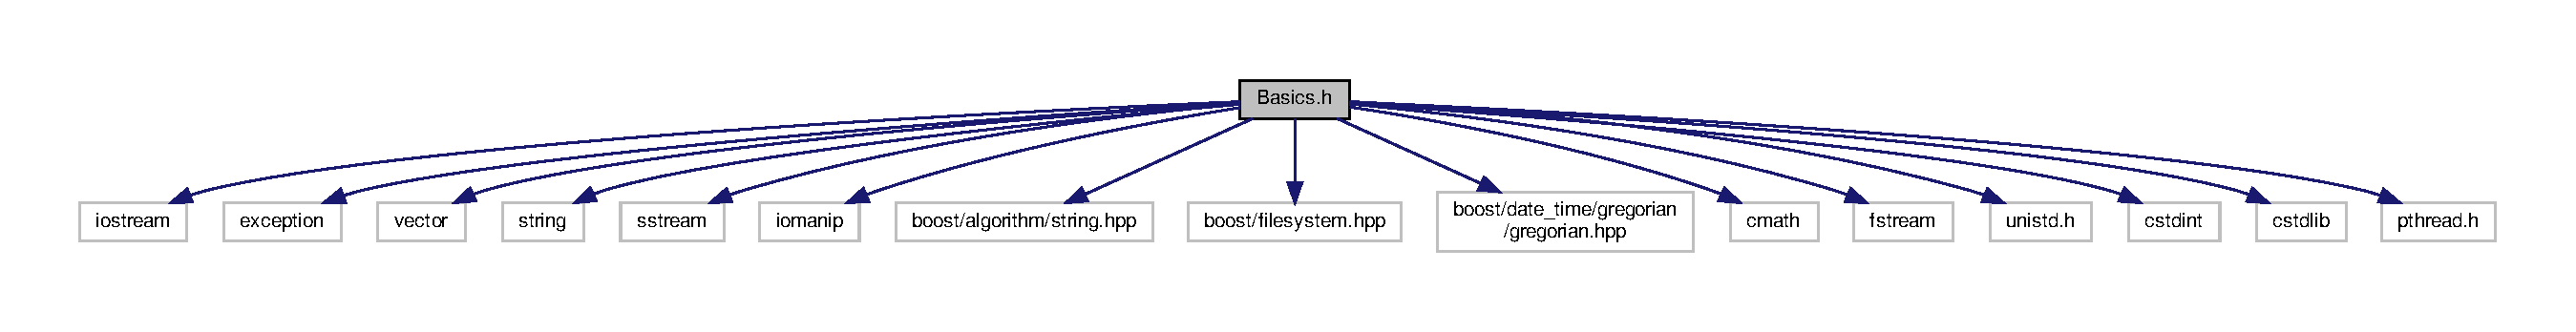
\includegraphics[width=350pt]{Basics_8h__incl}
\end{center}
\end{figure}
This graph shows which files directly or indirectly include this file\+:\nopagebreak
\begin{figure}[H]
\begin{center}
\leavevmode
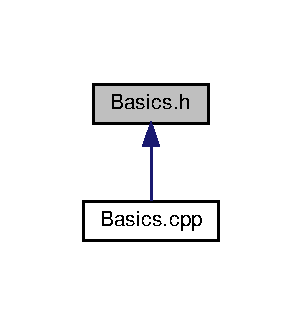
\includegraphics[width=350pt]{Basics_8h__dep__incl}
\end{center}
\end{figure}
\subsection*{Classes}
\begin{DoxyCompactItemize}
\item 
class \hyperlink{classCustomException}{Custom\+Exception}
\begin{DoxyCompactList}\small\item\em A class derived from standard class {\ttfamily std\+::exception}. \end{DoxyCompactList}\item 
struct \hyperlink{structTimeData}{Time\+Data}
\begin{DoxyCompactList}\small\item\em This structure is intended to store data related to {\itshape date} and {\itshape time} and to perform some operations with that data. \end{DoxyCompactList}\item 
struct \hyperlink{structFreqValues}{Freq\+Values}
\begin{DoxyCompactList}\small\item\em The aim of this structure is to store the curve of a determined parameter or variable versus the frequency, which is named a frequency curve here. \end{DoxyCompactList}\item 
struct \hyperlink{structSweep}{Sweep}
\begin{DoxyCompactList}\small\item\em The aim of this structure is to store the data points of a sweep obtained with the spectrum analyzer in a determined azimuth position, with a specific polarization. \end{DoxyCompactList}\item 
struct \hyperlink{structRFI}{R\+FI}
\begin{DoxyCompactList}\small\item\em The aim of this structure is to store the data related with the detected RF interference (\hyperlink{structRFI}{R\+FI})\+: frequency, power, azimuth angle, polarization, time, reference norm, etc. \end{DoxyCompactList}\item 
struct \hyperlink{structBandParameters}{Band\+Parameters}
\begin{DoxyCompactList}\small\item\em This structure is intended to store the parameters which are used to configure the spectrum analyzer in each frequency band. \end{DoxyCompactList}\end{DoxyCompactItemize}
\subsection*{Functions}
\begin{DoxyCompactItemize}
\item 
bool \hyperlink{Basics_8h_ab0cf00620947abc90fbfe36db36f8fc7}{approximately\+Equal} (float a, float b)
\begin{DoxyCompactList}\small\item\em Function intended to compare floating-\/point numbers as approximately equal, taking into account the floating-\/point rounding errors. \end{DoxyCompactList}\item 
bool \hyperlink{Basics_8h_adee734e43e4a9a5f4b9f610ccdd3f8e0}{approximately\+Equal} (std\+::vector$<$ float $>$ vectorA, std\+::vector$<$ float $>$ vectorB)
\begin{DoxyCompactList}\small\item\em Function intended to compare {\ttfamily std\+::vector$<$float$>$} containers as approximately equal, taking into account the floating-\/point rounding errors. \end{DoxyCompactList}\item 
std\+::vector$<$ float $>$ \hyperlink{Basics_8h_ac744212c600f3f610807ec4add576822}{operator-\/} (const std\+::vector$<$ float $>$ \&\hyperlink{Spectran_8h_a16fa8eb91a19fde7a399d85c521f63fd}{vect})
\begin{DoxyCompactList}\small\item\em An overloading of unary operator -\/ which negates the elements of a {\ttfamily std\+::vector$<$float$>$} container. \end{DoxyCompactList}\item 
\mbox{\Hypertarget{Basics_8h_abe6b1466ff5e3b09c33ca5dc9fc81c5a}\label{Basics_8h_abe6b1466ff5e3b09c33ca5dc9fc81c5a}} 
void \hyperlink{Basics_8h_abe6b1466ff5e3b09c33ca5dc9fc81c5a}{Wait\+For\+Key} ()
\begin{DoxyCompactList}\small\item\em This function stop the execution up to any key is pressed by the user and it was used for debugging purpose. \end{DoxyCompactList}\item 
\mbox{\Hypertarget{Basics_8h_adb434b11769fc3a9acd409f2fe534395}\label{Basics_8h_adb434b11769fc3a9acd409f2fe534395}} 
void \hyperlink{Basics_8h_adb434b11769fc3a9acd409f2fe534395}{Initialize\+G\+P\+IO} ()
\begin{DoxyCompactList}\small\item\em This function initializes all G\+P\+IO pins which are used for the input and output signals, in the way it is described in structure {\itshape pi\+Pins}. \end{DoxyCompactList}\item 
\mbox{\Hypertarget{Basics_8h_a37d643c013d8e020715ec625553673e7}\label{Basics_8h_a37d643c013d8e020715ec625553673e7}} 
void \hyperlink{Basics_8h_a37d643c013d8e020715ec625553673e7}{Turn\+Off\+Leds} ()
\begin{DoxyCompactList}\small\item\em The aim of this function is to turn all L\+E\+Ds off. \end{DoxyCompactList}\item 
void \hyperlink{Basics_8h_a2f7418278fcdac50f5c6a73744f8013c}{Turn\+On\+Front\+End} ()
\begin{DoxyCompactList}\small\item\em The aim of this function is to turn on the RF front-\/end elements in a sequential manner, from the spectrum analyzer to the antenna.. \end{DoxyCompactList}\item 
void \hyperlink{Basics_8h_a5ffe8b7dfe9c6702ed65b2b8b47bc3e1}{Turn\+Off\+Front\+End} ()
\begin{DoxyCompactList}\small\item\em The aim of this function is to turn off the RF front-\/end elements in a sequential manner, from the antenna to the spectrum analyzer. \end{DoxyCompactList}\item 
\mbox{\Hypertarget{Basics_8h_ae964ff8411b4fdcaf65cb5529aea4bef}\label{Basics_8h_ae964ff8411b4fdcaf65cb5529aea4bef}} 
void \hyperlink{Basics_8h_ae964ff8411b4fdcaf65cb5529aea4bef}{Print\+Help} ()
\begin{DoxyCompactList}\small\item\em This function prints in the {\ttfamily stdout} a message whit a software description and the descriptions of its arguments. \end{DoxyCompactList}\item 
bool \hyperlink{Basics_8h_abab505eef94a08a9092f916c62637071}{Process\+Main\+Arguments} (int argc, char $\ast$argv\mbox{[}$\,$\mbox{]})
\begin{DoxyCompactList}\small\item\em This function process the software\textquotesingle{}s arguments, which define the behavior of this one. \end{DoxyCompactList}\end{DoxyCompactItemize}
\subsection*{Variables}
\begin{DoxyCompactItemize}
\item 
\mbox{\Hypertarget{Basics_8h_a0423f4cb393331ce0b9f6b3a43adcaae}\label{Basics_8h_a0423f4cb393331ce0b9f6b3a43adcaae}} 
const std\+::string \hyperlink{Basics_8h_a0423f4cb393331ce0b9f6b3a43adcaae}{B\+A\+S\+E\+\_\+\+P\+A\+TH} = \char`\"{}/home/new-\/mauro/R\+F\+I\+MS-\/C\+A\+RT\char`\"{}
\begin{DoxyCompactList}\small\item\em This constant define the base path where there are the files and folders used by the software. \end{DoxyCompactList}\item 
\mbox{\Hypertarget{Basics_8h_a73be6649a1d91070309752a2fbcf5b8a}\label{Basics_8h_a73be6649a1d91070309752a2fbcf5b8a}} 
bool \hyperlink{Basics_8h_a73be6649a1d91070309752a2fbcf5b8a}{flag\+Cal\+Enabled}
\begin{DoxyCompactList}\small\item\em The declaration of an external flag which defines if the calibration of the RF front end must be done or not. \end{DoxyCompactList}\item 
\mbox{\Hypertarget{Basics_8h_a20c207881b1f505ca91715905e27bacb}\label{Basics_8h_a20c207881b1f505ca91715905e27bacb}} 
bool \hyperlink{Basics_8h_a20c207881b1f505ca91715905e27bacb}{flag\+Plot}
\begin{DoxyCompactList}\small\item\em The declaration of an external flag which defines if the software has to generate plots. \end{DoxyCompactList}\item 
\mbox{\Hypertarget{Basics_8h_a6f3cbd74619175fd2b8580b37587f825}\label{Basics_8h_a6f3cbd74619175fd2b8580b37587f825}} 
bool \hyperlink{Basics_8h_a6f3cbd74619175fd2b8580b37587f825}{flag\+Infinite\+Loop}
\begin{DoxyCompactList}\small\item\em The declaration of an external flag which defines if the software has to perform a finite number of measurement cycles or iterate infinitely. \end{DoxyCompactList}\item 
\mbox{\Hypertarget{Basics_8h_a816d4b897ea7e7b008ad3957e2203934}\label{Basics_8h_a816d4b897ea7e7b008ad3957e2203934}} 
bool \hyperlink{Basics_8h_a816d4b897ea7e7b008ad3957e2203934}{flag\+R\+FI}
\begin{DoxyCompactList}\small\item\em The declaration of an external flag which defines if the software has to perform \hyperlink{structRFI}{R\+FI} detection or not. \end{DoxyCompactList}\item 
\mbox{\Hypertarget{Basics_8h_a7616186dd32bbd21eb512dfdc580214c}\label{Basics_8h_a7616186dd32bbd21eb512dfdc580214c}} 
bool \hyperlink{Basics_8h_a7616186dd32bbd21eb512dfdc580214c}{flag\+Upload}
\begin{DoxyCompactList}\small\item\em The declaration of an external flag which defines if the software has to upload the measurements or not. \end{DoxyCompactList}\item 
unsigned int \hyperlink{Basics_8h_a4a22fc28d7ca5b183f4a901f4dafd4a6}{num\+Of\+Meas\+Cycles}
\begin{DoxyCompactList}\small\item\em The declaration of an external variable which stores the number of measurements cycles which left to be done. It is used when the user wishes a finite number of measurements cycles. \end{DoxyCompactList}\item 
\hyperlink{structRFI_a18cfa7d24274bbcd14acc6b513860cb0}{R\+F\+I\+::\+Thresholds\+Norm} \hyperlink{Basics_8h_a5fca012de3aeabad258f4f0fa6877334}{rfi\+Norm}
\begin{DoxyCompactList}\small\item\em The declaration of an external variable which saves the norm which defines the harmful interference levels\+: ska-\/mode1, ska-\/mode2, itu-\/ra769-\/2-\/vlbi. \end{DoxyCompactList}\end{DoxyCompactItemize}


\subsection{Detailed Description}
This header file contains the declarations of the most basic and global entities which are used by many others entities. 

This header file contains the declarations and definitions of the following\+:
\begin{DoxyItemize}
\item Preprocessor definitions ({\ttfamily define})\+: these elements define the blocks of code will be taking into account by the compiler, so the way the software will behave after the compilation and linking.
\item Global libraries, i.\+e. the libraries which are used by several functions and classes from different files.
\item Global constants and variables.
\item Global structures which are used to interchange data between different objects and functions.
\item Global structures which contain common data to all software\textquotesingle{}s entities.
\item A global class to handle exceptions.
\item Global functions which are used in several different places. \begin{DoxyAuthor}{Author}
Mauro Diamantino 
\end{DoxyAuthor}

\end{DoxyItemize}

\subsection{Function Documentation}
\mbox{\Hypertarget{Basics_8h_ab0cf00620947abc90fbfe36db36f8fc7}\label{Basics_8h_ab0cf00620947abc90fbfe36db36f8fc7}} 
\index{Basics.\+h@{Basics.\+h}!approximately\+Equal@{approximately\+Equal}}
\index{approximately\+Equal@{approximately\+Equal}!Basics.\+h@{Basics.\+h}}
\subsubsection{\texorpdfstring{approximately\+Equal()}{approximatelyEqual()}\hspace{0.1cm}{\footnotesize\ttfamily [1/2]}}
{\footnotesize\ttfamily bool approximately\+Equal (\begin{DoxyParamCaption}\item[{float}]{a,  }\item[{float}]{b }\end{DoxyParamCaption})}



Function intended to compare floating-\/point numbers as approximately equal, taking into account the floating-\/point rounding errors. 

This function was copied from this \href{https://www.learncpp.com/cpp-tutorial/35-relational-operators-comparisons/}{\tt link}, but it was modified. It is based in the Knuth’s algorithm but it uses two epsilons, an absolute epsilon (A\+B\+S\+\_\+\+E\+P\+S\+I\+L\+ON) which is very small and is intended to compare near-\/zero floating-\/point numbers and a relative epsilon (R\+E\+L\+\_\+\+E\+P\+S\+I\+L\+ON, which is a percentage of the biggest operand) to compare the rest of the floating-\/point numbers. The function returns true if the difference between a and b is less than A\+B\+S\+\_\+\+E\+P\+S\+I\+L\+ON, or within R\+E\+L\+\_\+\+E\+P\+S\+I\+L\+ON percent of the larger of a and b. 
\begin{DoxyParams}[1]{Parameters}
\mbox{\tt in}  & {\em a} & The left-\/hand side argument. \\
\hline
\mbox{\tt in}  & {\em b} & The right-\/hand side argument. \\
\hline
\end{DoxyParams}
\mbox{\Hypertarget{Basics_8h_adee734e43e4a9a5f4b9f610ccdd3f8e0}\label{Basics_8h_adee734e43e4a9a5f4b9f610ccdd3f8e0}} 
\index{Basics.\+h@{Basics.\+h}!approximately\+Equal@{approximately\+Equal}}
\index{approximately\+Equal@{approximately\+Equal}!Basics.\+h@{Basics.\+h}}
\subsubsection{\texorpdfstring{approximately\+Equal()}{approximatelyEqual()}\hspace{0.1cm}{\footnotesize\ttfamily [2/2]}}
{\footnotesize\ttfamily bool approximately\+Equal (\begin{DoxyParamCaption}\item[{std\+::vector$<$ float $>$}]{vectorA,  }\item[{std\+::vector$<$ float $>$}]{vectorB }\end{DoxyParamCaption})}



Function intended to compare {\ttfamily std\+::vector$<$float$>$} containers as approximately equal, taking into account the floating-\/point rounding errors. 

This function is based on the function presented in this \href{https://www.learncpp.com/cpp-tutorial/35-relational-operators-comparisons/}{\tt link}.

It is based in the Knuth’s algorithm but it uses two epsilons, an absolute epsilon (A\+B\+S\+\_\+\+E\+P\+S\+I\+L\+ON) which is very small and is intended to compare near-\/zero floating-\/point numbers and a relative epsilon (R\+E\+L\+\_\+\+E\+P\+S\+I\+L\+ON, which is a percentage of the biggest operand) to compare the rest of the floating-\/point numbers. The function returns true if the difference between a and b is less than A\+B\+S\+\_\+\+E\+P\+S\+I\+L\+ON, or within R\+E\+L\+\_\+\+E\+P\+S\+I\+L\+ON percent of the larger of a and b. 
\begin{DoxyParams}[1]{Parameters}
\mbox{\tt in}  & {\em vectorA} & The left-\/hand side argument. \\
\hline
\mbox{\tt in}  & {\em vectorB} & The right-\/hand side argument. \\
\hline
\end{DoxyParams}
\mbox{\Hypertarget{Basics_8h_ac744212c600f3f610807ec4add576822}\label{Basics_8h_ac744212c600f3f610807ec4add576822}} 
\index{Basics.\+h@{Basics.\+h}!operator-\/@{operator-\/}}
\index{operator-\/@{operator-\/}!Basics.\+h@{Basics.\+h}}
\subsubsection{\texorpdfstring{operator-\/()}{operator-()}}
{\footnotesize\ttfamily std\+::vector$<$float$>$ operator-\/ (\begin{DoxyParamCaption}\item[{const std\+::vector$<$ float $>$ \&}]{vect }\end{DoxyParamCaption})}



An overloading of unary operator -\/ which negates the elements of a {\ttfamily std\+::vector$<$float$>$} container. 


\begin{DoxyParams}[1]{Parameters}
\mbox{\tt in}  & {\em vect} & A {\ttfamily std\+::vector$<$float$>$} container which must be negated. \\
\hline
\end{DoxyParams}
\mbox{\Hypertarget{Basics_8h_abab505eef94a08a9092f916c62637071}\label{Basics_8h_abab505eef94a08a9092f916c62637071}} 
\index{Basics.\+h@{Basics.\+h}!Process\+Main\+Arguments@{Process\+Main\+Arguments}}
\index{Process\+Main\+Arguments@{Process\+Main\+Arguments}!Basics.\+h@{Basics.\+h}}
\subsubsection{\texorpdfstring{Process\+Main\+Arguments()}{ProcessMainArguments()}}
{\footnotesize\ttfamily bool Process\+Main\+Arguments (\begin{DoxyParamCaption}\item[{int}]{argc,  }\item[{char $\ast$}]{argv\mbox{[}$\,$\mbox{]} }\end{DoxyParamCaption})}



This function process the software\textquotesingle{}s arguments, which define the behavior of this one. 

This function determines the values of the behavior flags (flag\+Cal\+Enabled, flag\+Plot, flag\+R\+FI, etc.) taking into account the arguments that were received and its values. The function returns a {\ttfamily true} value if the arguments were processed correctly and a {\ttfamily false} value if there was an argument which could not be recognized, and in that case it presents a message, in the {\ttfamily stdout}, explaining the correct use of the software arguments. 
\begin{DoxyParams}[1]{Parameters}
\mbox{\tt in}  & {\em argc} & The number of arguments that were received by the software. \\
\hline
\mbox{\tt in}  & {\em argv} & An array of C strings ({\ttfamily char$\ast$}) where each one is a software\textquotesingle{}s argument. \\
\hline
\end{DoxyParams}
\mbox{\Hypertarget{Basics_8h_a5ffe8b7dfe9c6702ed65b2b8b47bc3e1}\label{Basics_8h_a5ffe8b7dfe9c6702ed65b2b8b47bc3e1}} 
\index{Basics.\+h@{Basics.\+h}!Turn\+Off\+Front\+End@{Turn\+Off\+Front\+End}}
\index{Turn\+Off\+Front\+End@{Turn\+Off\+Front\+End}!Basics.\+h@{Basics.\+h}}
\subsubsection{\texorpdfstring{Turn\+Off\+Front\+End()}{TurnOffFrontEnd()}}
{\footnotesize\ttfamily void Turn\+Off\+Front\+End (\begin{DoxyParamCaption}{ }\end{DoxyParamCaption})}



The aim of this function is to turn off the RF front-\/end elements in a sequential manner, from the antenna to the spectrum analyzer. 

To turn off the RF front-\/end elements sequentially, this function begins ensuring the noise source is turned off, then it switches the input to that device, it waits 1 second, it turns the L\+N\+As off, it waits again 1 second and, finally, it turns the spectrum analyzer off. \mbox{\Hypertarget{Basics_8h_a2f7418278fcdac50f5c6a73744f8013c}\label{Basics_8h_a2f7418278fcdac50f5c6a73744f8013c}} 
\index{Basics.\+h@{Basics.\+h}!Turn\+On\+Front\+End@{Turn\+On\+Front\+End}}
\index{Turn\+On\+Front\+End@{Turn\+On\+Front\+End}!Basics.\+h@{Basics.\+h}}
\subsubsection{\texorpdfstring{Turn\+On\+Front\+End()}{TurnOnFrontEnd()}}
{\footnotesize\ttfamily void Turn\+On\+Front\+End (\begin{DoxyParamCaption}{ }\end{DoxyParamCaption})}



The aim of this function is to turn on the RF front-\/end elements in a sequential manner, from the spectrum analyzer to the antenna.. 

To turn on the RF front-\/end elements in a sequential manner, first, this function turns the spectrum analyzer on, then it waits 5 seconds, it turns the L\+N\+As on, it waits again but this time just 1 second and, finally, it switches the input to the antenna. 

\subsection{Variable Documentation}
\mbox{\Hypertarget{Basics_8h_a4a22fc28d7ca5b183f4a901f4dafd4a6}\label{Basics_8h_a4a22fc28d7ca5b183f4a901f4dafd4a6}} 
\index{Basics.\+h@{Basics.\+h}!num\+Of\+Meas\+Cycles@{num\+Of\+Meas\+Cycles}}
\index{num\+Of\+Meas\+Cycles@{num\+Of\+Meas\+Cycles}!Basics.\+h@{Basics.\+h}}
\subsubsection{\texorpdfstring{num\+Of\+Meas\+Cycles}{numOfMeasCycles}}
{\footnotesize\ttfamily unsigned int num\+Of\+Meas\+Cycles}



The declaration of an external variable which stores the number of measurements cycles which left to be done. It is used when the user wishes a finite number of measurements cycles. 

The declaration of an external variable which stores the number of measurements cycles which left to be done. It is used when the user wishes a finite number of measurements cycles. \mbox{\Hypertarget{Basics_8h_a5fca012de3aeabad258f4f0fa6877334}\label{Basics_8h_a5fca012de3aeabad258f4f0fa6877334}} 
\index{Basics.\+h@{Basics.\+h}!rfi\+Norm@{rfi\+Norm}}
\index{rfi\+Norm@{rfi\+Norm}!Basics.\+h@{Basics.\+h}}
\subsubsection{\texorpdfstring{rfi\+Norm}{rfiNorm}}
{\footnotesize\ttfamily \hyperlink{structRFI_a18cfa7d24274bbcd14acc6b513860cb0}{R\+F\+I\+::\+Thresholds\+Norm} rfi\+Norm}



The declaration of an external variable which saves the norm which defines the harmful interference levels\+: ska-\/mode1, ska-\/mode2, itu-\/ra769-\/2-\/vlbi. 

The declaration of an external variable which saves the norm which defines the harmful interference levels\+: ska-\/mode1, ska-\/mode2, itu-\/ra769-\/2-\/vlbi. 
%--- End generated contents ---

% Index
\backmatter
\newpage
\phantomsection
\clearemptydoublepage
\addcontentsline{toc}{chapter}{Index}
\printindex

\end{document}
